\documentclass[10pt]{article}  

%%%%%%%% PREÁMBULO %%%%%%%%%%%%
\title{Plantilla para prácticas de UGR}
\usepackage[spanish]{babel} %Indica que escribiermos en español
\usepackage[utf8]{inputenc} %Indica qué codificación se está usando ISO-8859-1(latin1)  o utf8  
\usepackage{amsmath} % Comandos extras para matemáticas (cajas para ecuaciones,
% etc)
\usepackage{amssymb} % Simbolos matematicos (por lo tanto)
\usepackage{graphicx} % Incluir imágenes en LaTeX
\usepackage{color} % Para colorear texto
\usepackage{subfigure} % subfiguras
\usepackage{float} %Podemos usar el especificador [H] en las figuras para que se
% queden donde queramos
\usepackage{capt-of} % Permite usar etiquetas fuera de elementos flotantes
% (etiquetas de figuras)
\usepackage{sidecap} % Para poner el texto de las imágenes al lado
	\sidecaptionvpos{figure}{c} % Para que el texto se alinie al centro vertical
\usepackage{caption} % Para poder quitar numeracion de figuras
\usepackage{commath} % funcionalidades extras para diferenciales, integrales,
% etc (\od, \dif, etc)
\usepackage{cancel} % para cancelar expresiones (\cancelto{0}{x})

\graphicspath{{/Users/jesusgarciamanday/Desktop/Master/CC-II/Practicas/Practica2/p2/Imagenes/}}

\usepackage{anysize} 					% Para personalizar el ancho de  los márgenes
\marginsize{2cm}{2cm}{2cm}{2cm} % Izquierda, derecha, arriba, abajo

\usepackage{appendix}
\renewcommand{\appendixname}{Apéndices}
\renewcommand{\appendixtocname}{Apéndices}
\renewcommand{\appendixpagename}{Apéndices} 

% Para que las referencias sean hipervínculos a las figuras o ecuaciones y
% aparezcan en color
\usepackage[colorlinks=true,plainpages=true,citecolor=blue,linkcolor=blue]{hyperref}
%\usepackage{hyperref} 
% Para agregar encabezado y pie de página
\usepackage{fancyhdr} 
\pagestyle{fancy}
\fancyhf{}
\fancyhead[L]{\footnotesize UGR} %encabezado izquierda
\fancyhead[R]{\footnotesize CCIA}   % dereecha
\fancyfoot[R]{\footnotesize Pr\'actica 2 - Docker }  % Pie derecha
\fancyfoot[C]{\thepage}  % centro
\fancyfoot[L]{\footnotesize Master en Ingenier\'ia Inform\'atica }  %izquierda
\renewcommand{\footrulewidth}{0.4pt}


\usepackage{listings} % Para usar código fuente
\definecolor{dkgreen}{rgb}{0,0.6,0} % Definimos colores para usar en el código
\definecolor{gray}{rgb}{0.5,0.5,0.5} 
% configuración para el lenguaje que queramos utilizar
\lstset{language=Matlab,
   keywords={break,case,catch,continue,else,elseif,end,for,function,
      global,if,otherwise,persistent,return,switch,try,while},
   basicstyle=\ttfamily,
   keywordstyle=\color{blue},
   commentstyle=\color{red},
   stringstyle=\color{dkgreen},
   numbers=left,
   numberstyle=\tiny\color{gray},
   stepnumber=1,
   numbersep=10pt,
   backgroundcolor=\color{white},
   tabsize=4,
   showspaces=false,
   showstringspaces=false}

\newcommand{\sen}{\operatorname{\sen}}	% Definimos el comando \sen para el seno
%en español

\title{Práctica 2 - Docker}

%%%%%%%% TERMINA PREÁMBULO %%%%%%%%%%%%

\begin{document}

%%%%%%%%%%%%%%%%%%%%%%%%%%%%%%%%%% PORTADA %%%%%%%%%%%%%%%%%%%%%%%%%%%%%%%%%%%%%%%%%%%%
																					%%%
\begin{center}																		%%%
\newcommand{\HRule}{\rule{\linewidth}{0.5mm}}									%%%\left
 																					%%%
\begin{minipage}{0.48\textwidth} \begin{flushleft}
%
\includegraphics[scale = 0.63]{Imagenes/logo_upiita}
\end{flushleft}\end{minipage}
\begin{minipage}{0.48\textwidth} \begin{flushright}
%
\includegraphics[scale = 0.35]{Imagenes/IPN}
\end{flushright}\end{minipage}

													 								%%%
\vspace*{-1.5cm}								%%%
																					%%%	
\textsc{\huge Universidad de\\ \vspace{5px} Granada}\\[1.5cm]	

\textsc{\LARGE Master Profesional en Ingenier\'ia Inform\'atica }\\[1.5cm]													%%%

\begin{minipage}{0.9\textwidth} 
\begin{center}																					%%%
\textsc{\LARGE Pr\'actica 2}
\end{center}
\end{minipage}\\[0.5cm]
%%%
    																				%%%
 			\vspace*{1cm}																		%%%
																					%%%
\HRule \\[0.4cm]																	%%%
{ \huge \bfseries Docker}\\[0.4cm]	%%%
 																					%%%
\HRule \\[1.5cm]																	%%%
 																				%%%
																					%%%
\begin{minipage}{0.46\textwidth}													%%%
\begin{flushleft} \large															%%%
\emph{Autor:}\\	
Manuel Jes\'us Garc\'ia Manday (nickter@correo.ugr.es)\\
%%%
			%\vspace*{2cm}	
            													%%%
										 						%%%
\end{flushleft}																		%%%
\end{minipage}		
																%%%
\begin{minipage}{0.52\textwidth}		
\vspace{-0.6cm}											%%%
\begin{flushright} \large															%%%
													%%%
\end{flushright}																	%%%
\end{minipage}	
\vspace*{1cm}
%\begin{flushleft}
 	
%\end{flushleft}
%%%
 		\flushleft{\textbf{\Large Master en Ingenier\'ia Inform\'atica}	}\\																		%%%
\vspace{2cm} 																				
\begin{center}																					
{\large \today}																	%%%
 			\end{center}												  						
\end{center}							 											
																					
\newpage																		
%%%%%%%%%%%%%%%%%%%% TERMINA PORTADA %%%%%%%%%%%%%%%%%%%%%%%%%%%%%%%%

\tableofcontents 

\newpage

\section{Objetivo.}



El objetivo de esta práctica es familiarizarse con el uso de una plataforma PaaS y desarrollar habilidades de despliegue de contenedores y configurar aplicaciones sencillas en los mismos.\\



\section{Descripción general del despliegue de un contenedor en docker.} 

Lo primero que se debe realizar es una conexión remota hacia el servidor hadoop.ugr.es y comprobar que el acceso a docker es correcto.\\

\begin{figure}[H]
	\begin{center}
 		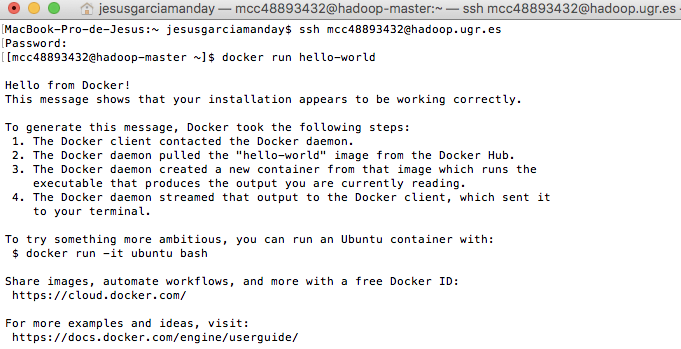
\includegraphics[width = 0.75\textwidth]{p2-img1}
 		\captionof{figure}{\label{fig:IPN}Conexión ssh y prueba del sistema docker.} 
	\end{center} 
\end{figure}

Una vez que hemos comprobado el funcionamiento del sistema docker, lo siguiente será buscar si ya existe alguna imagen en el sistema que cumpla los requisitos que buscamos, es decir, que tenga los servicios de \textbf{APACHE, SSL} y \textbf{PHP5} instalados como se solicita para el primer contenedor. Para ello vamos a utilizar el comando \textbf{docker search} y a continuación el nombre de los servicios que queremos que traiga la imagen incorporados como se muestra en la siguiente figura.\\

\begin{figure}[H]
	\begin{center}
 		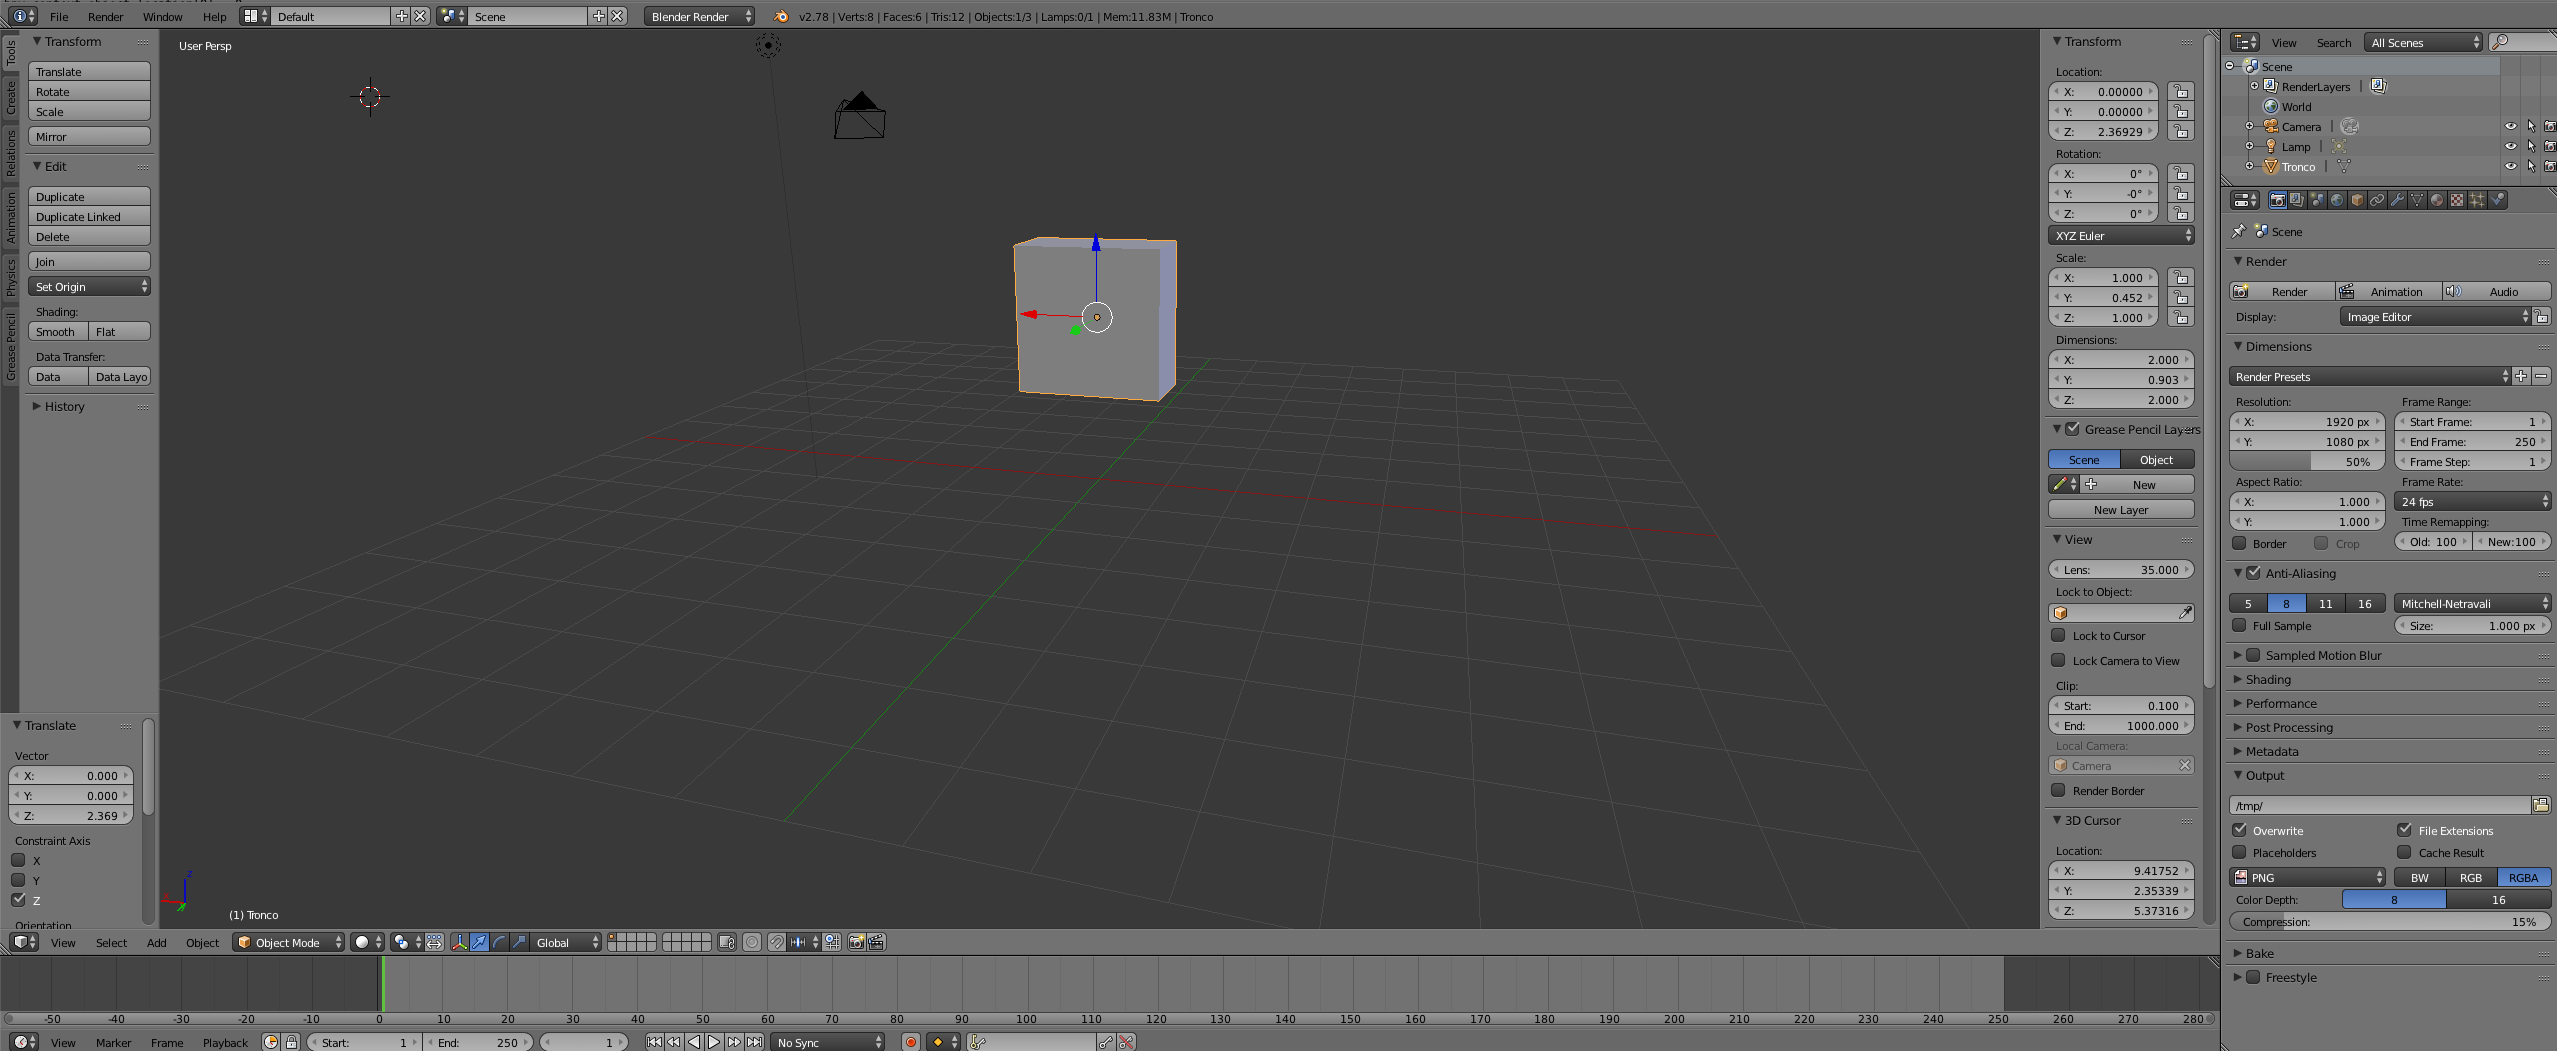
\includegraphics[width = 0.75\textwidth]{p2-img2}
 		\captionof{figure}{\label{fig:IPN}Buscando imagenes en docker.} 
	\end{center} 
\end{figure}

Como se puede apreciar en la anterior fotografía, la imagen \textbf{nimmis/apache-php5} cumple con los requisitos necesarios para crear el primer contenedor, por lo que lo siguiente que haremos será crearlo con el comando \textbf{docker run}. Cabe recordar que el puerto SSL por defecto es el 443, y que dicho servicio se instala con  \textbf{APACHE}, por lo que para redirigirlo al puerto asignado en el host anfritión hay que indicarlo mediante el flag \textbf{p} como se muestra en la imagen de a continuación. \\

\begin{figure}[H]
	\begin{center}
 		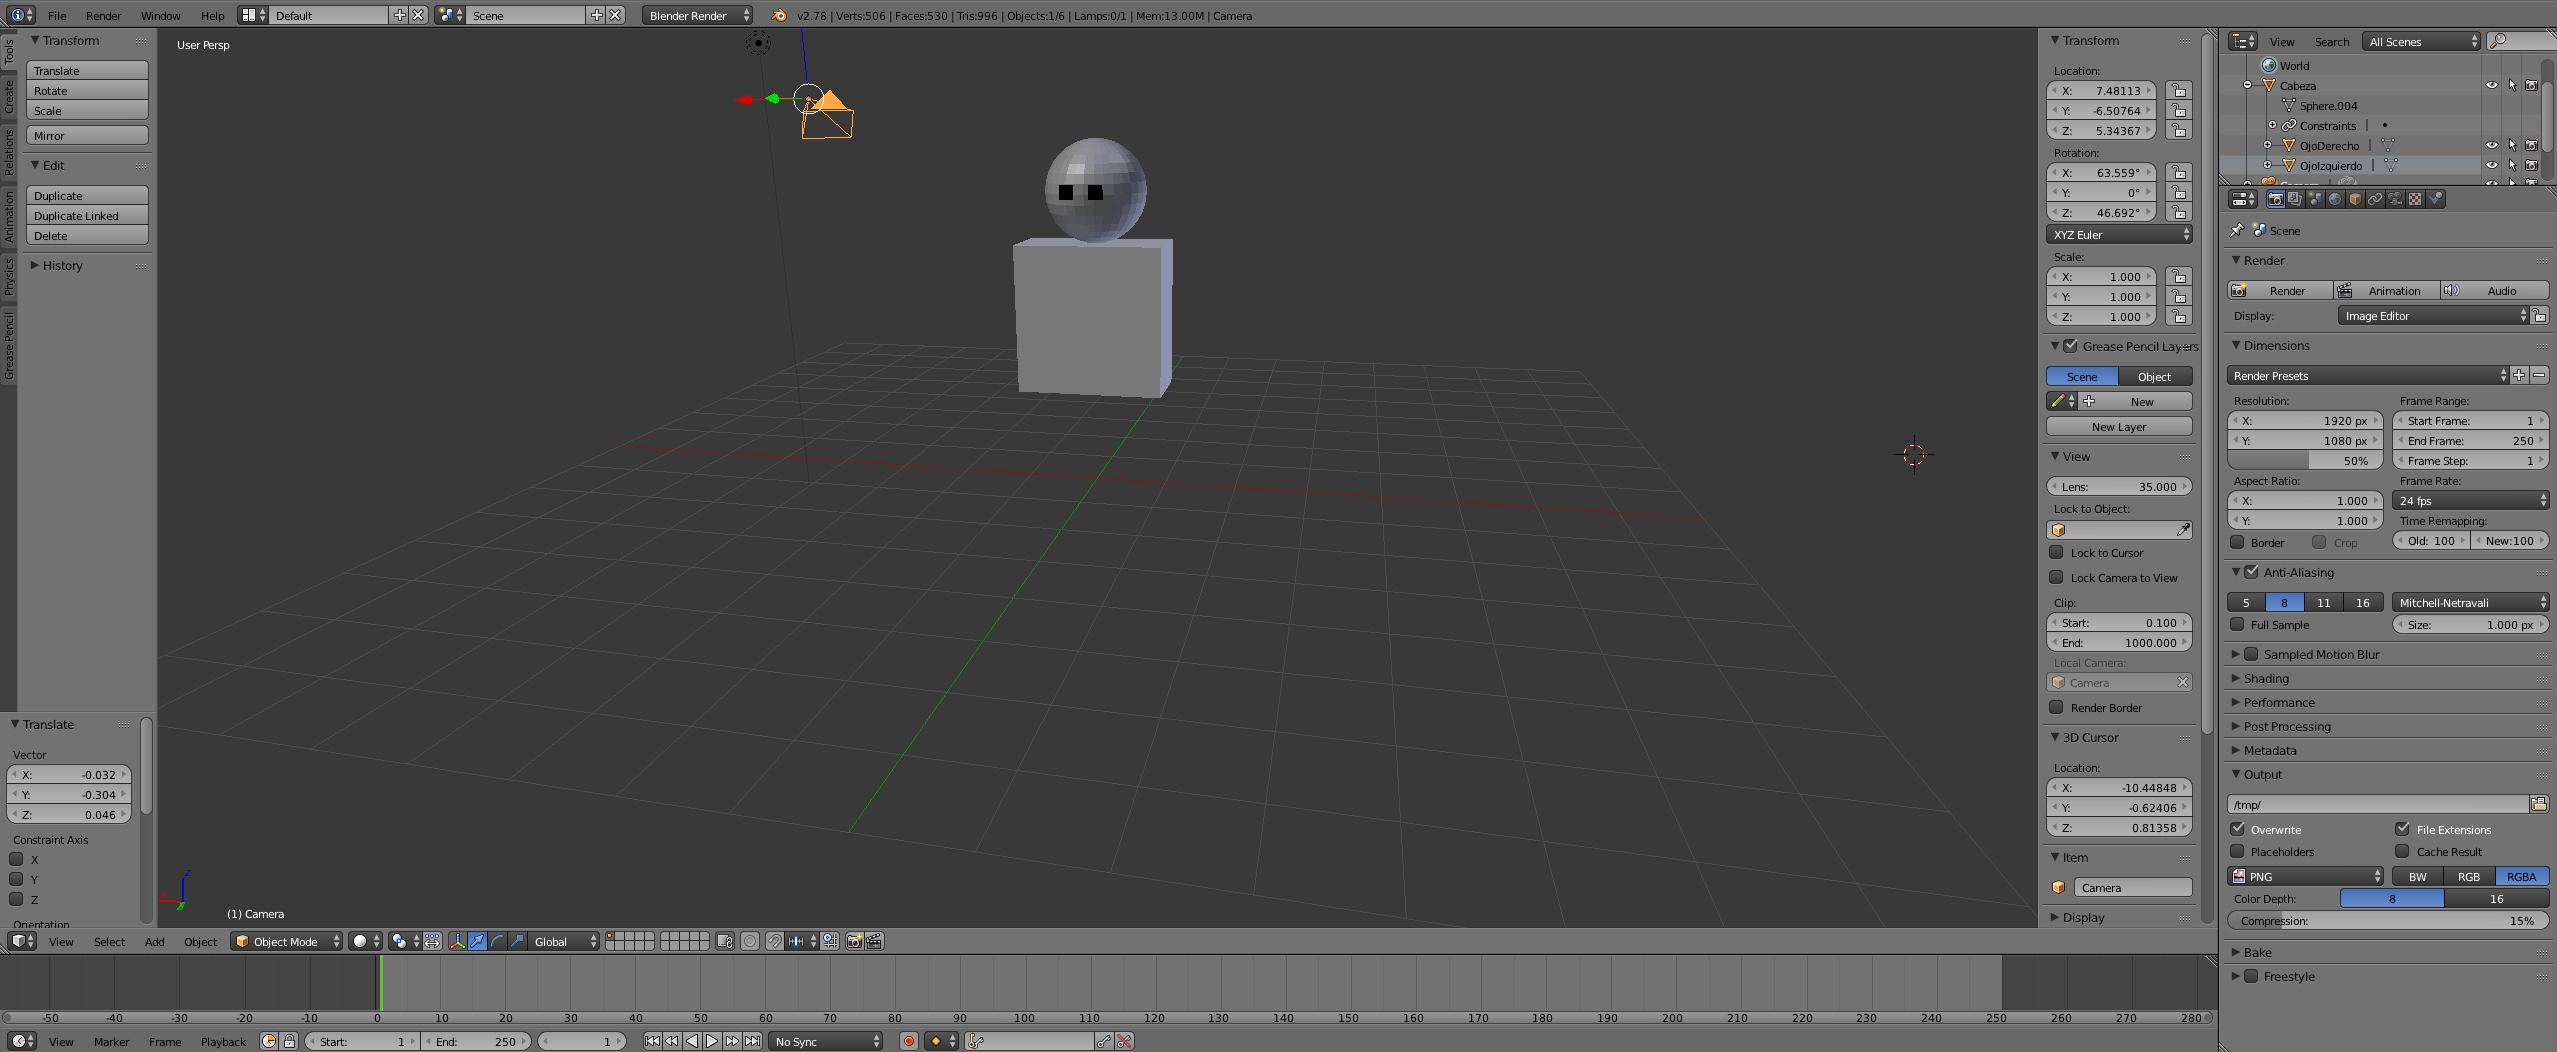
\includegraphics[width = 0.75\textwidth]{p2-img3}
 		\captionof{figure}{\label{fig:IPN}Creando el primer contenedor.} 
	\end{center} 
\end{figure}

Una vez creado el contenedor pasamos a comprobar que se ha realizado correctamente ejecutando el comando \textbf{docker ps}, el cual nos lista los contenedores creados sin errores en el sistema con atributos como el nombre, el redireccionamiento de puertos entre el host anfritión y el contenedor, etc. En la siguiente imagen se refelja.\\

\begin{figure}[H]
	\begin{center}
 		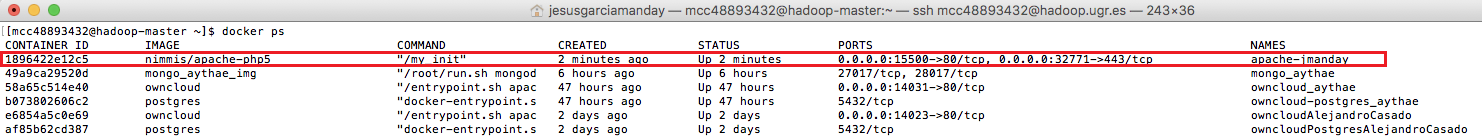
\includegraphics[width = 0.75\textwidth]{p2-img4}
 		\captionof{figure}{\label{fig:IPN}Comprobando que se ha creado el primer contenedor.} 
	\end{center} 
\end{figure}

Viendo que el contenedor se ha creado correctamente, ahora vamos a lanzarlo y acceder a su terminal para poder comprobar que tiene los servicios de \textbf{apache} y \textbf{php} instalados. Para realizar este paso vamos a emplear el comando \textbf{docker run} a través del cual se despliega un contenedor, pudiendole indicar un comando o acción a realizar por este. \\

\begin{figure}[H]
	\begin{center}
 		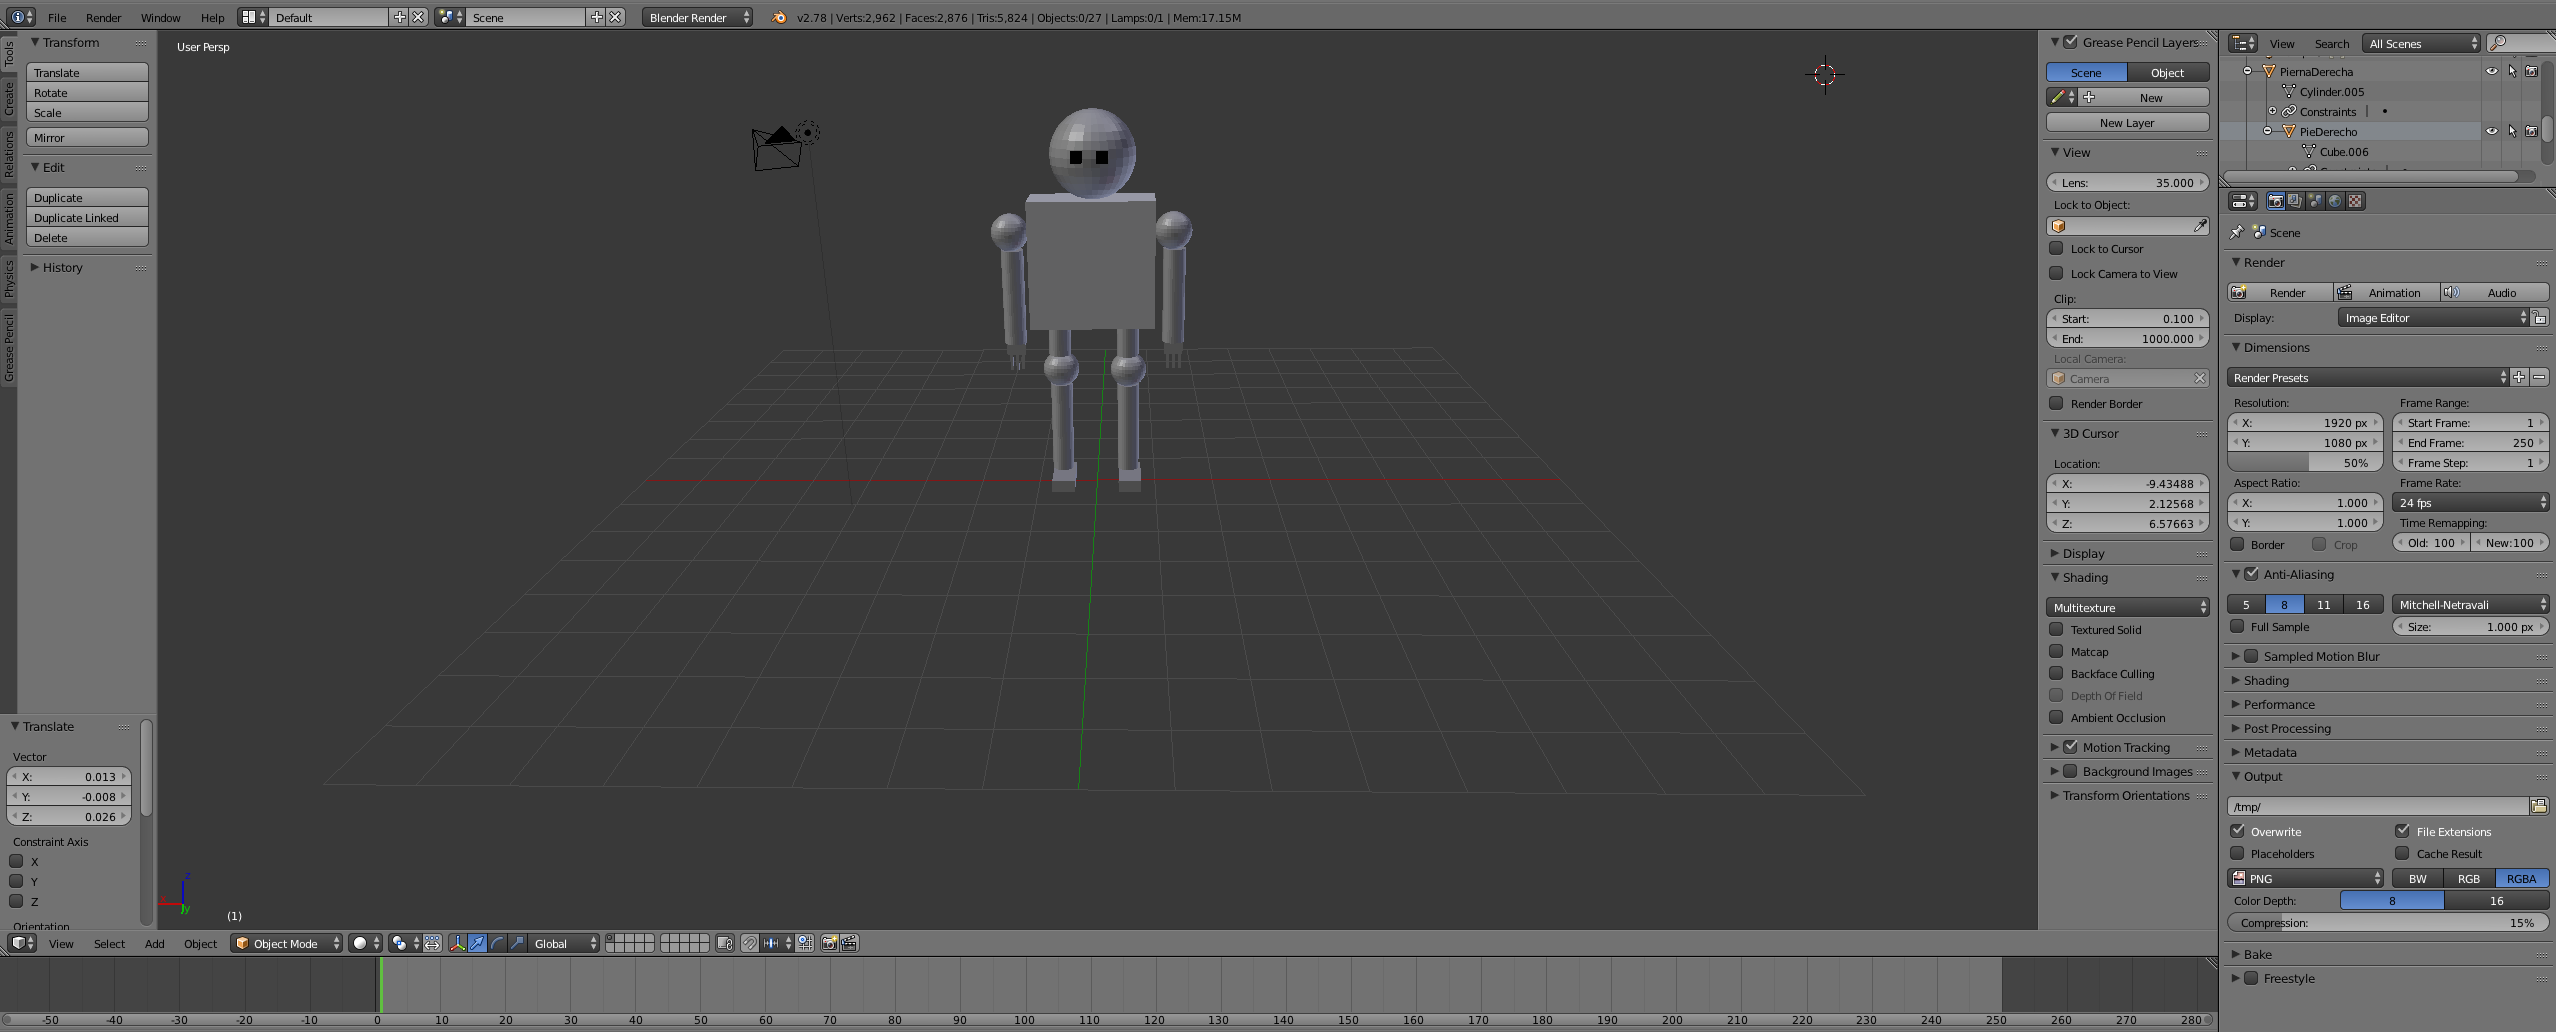
\includegraphics[width = 0.75\textwidth]{p2-img5}
 		\captionof{figure}{\label{fig:IPN}Lanzando el primer contenedor.} 
	\end{center} 
\end{figure}

\begin{figure}[H]
	\begin{center}
 		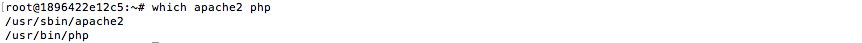
\includegraphics[width = 0.75\textwidth]{p2-img6}
 		\captionof{figure}{\label{fig:IPN}Comprobando que apache y php están instalados.} 
	\end{center} 
\end{figure}

\begin{figure}[H]
	\begin{center}
 		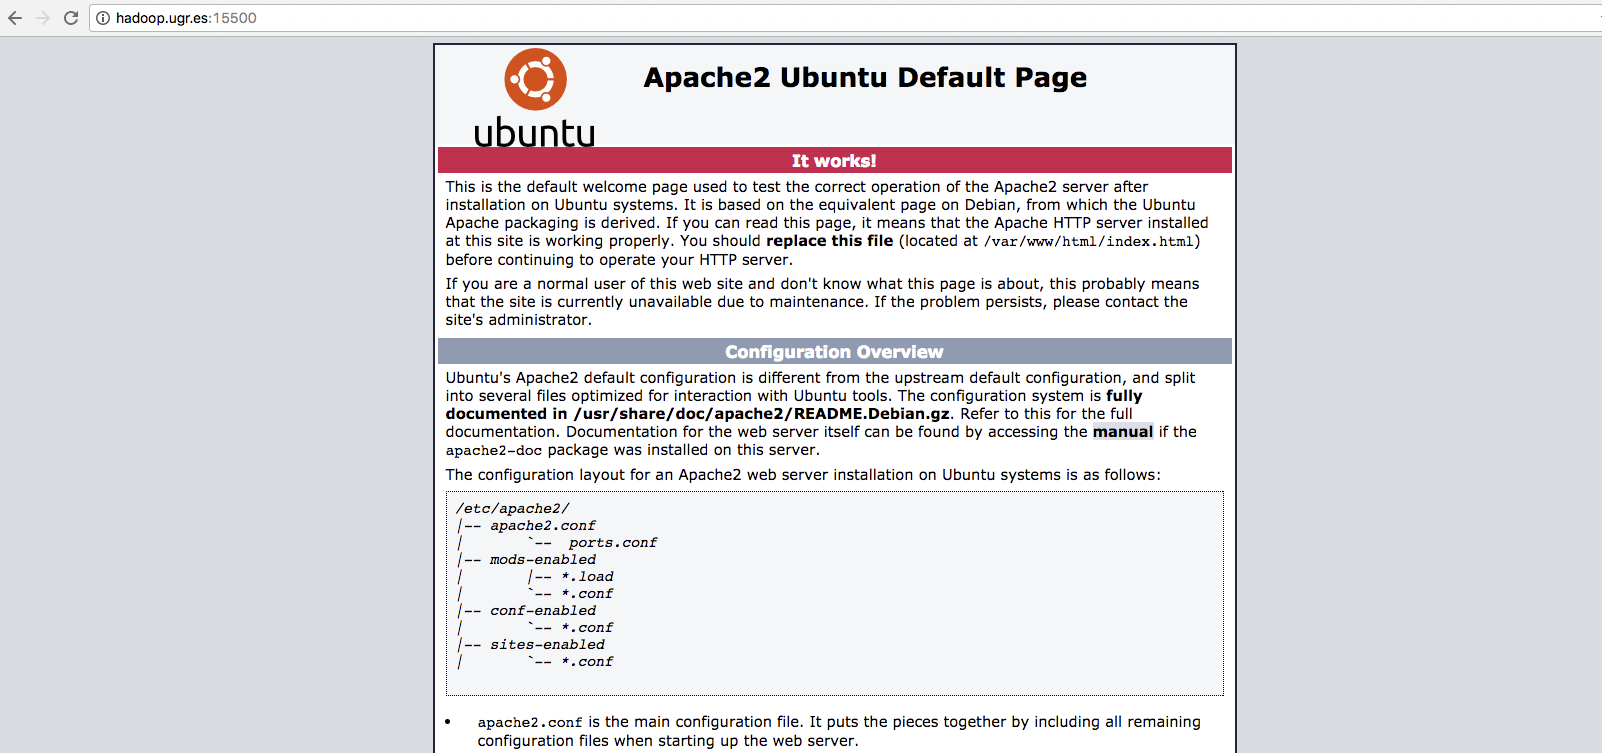
\includegraphics[width = 0.75\textwidth]{p2-img7}
 		\captionof{figure}{\label{fig:IPN}Comprobando apache.} 
	\end{center} 
\end{figure}

Para crear el segundo contenedor se van a seguir los mismos pasos que para el primero, por lo que lo primero que se realizará será buscar si existe alguna imagen en \textbf{Docker} con \textbf{MySQL} y si es así crearlo, lanzarlo y comprobar que el servicio de mysql existe en el contenedor.\\

\begin{figure}[H]
	\begin{center}
 		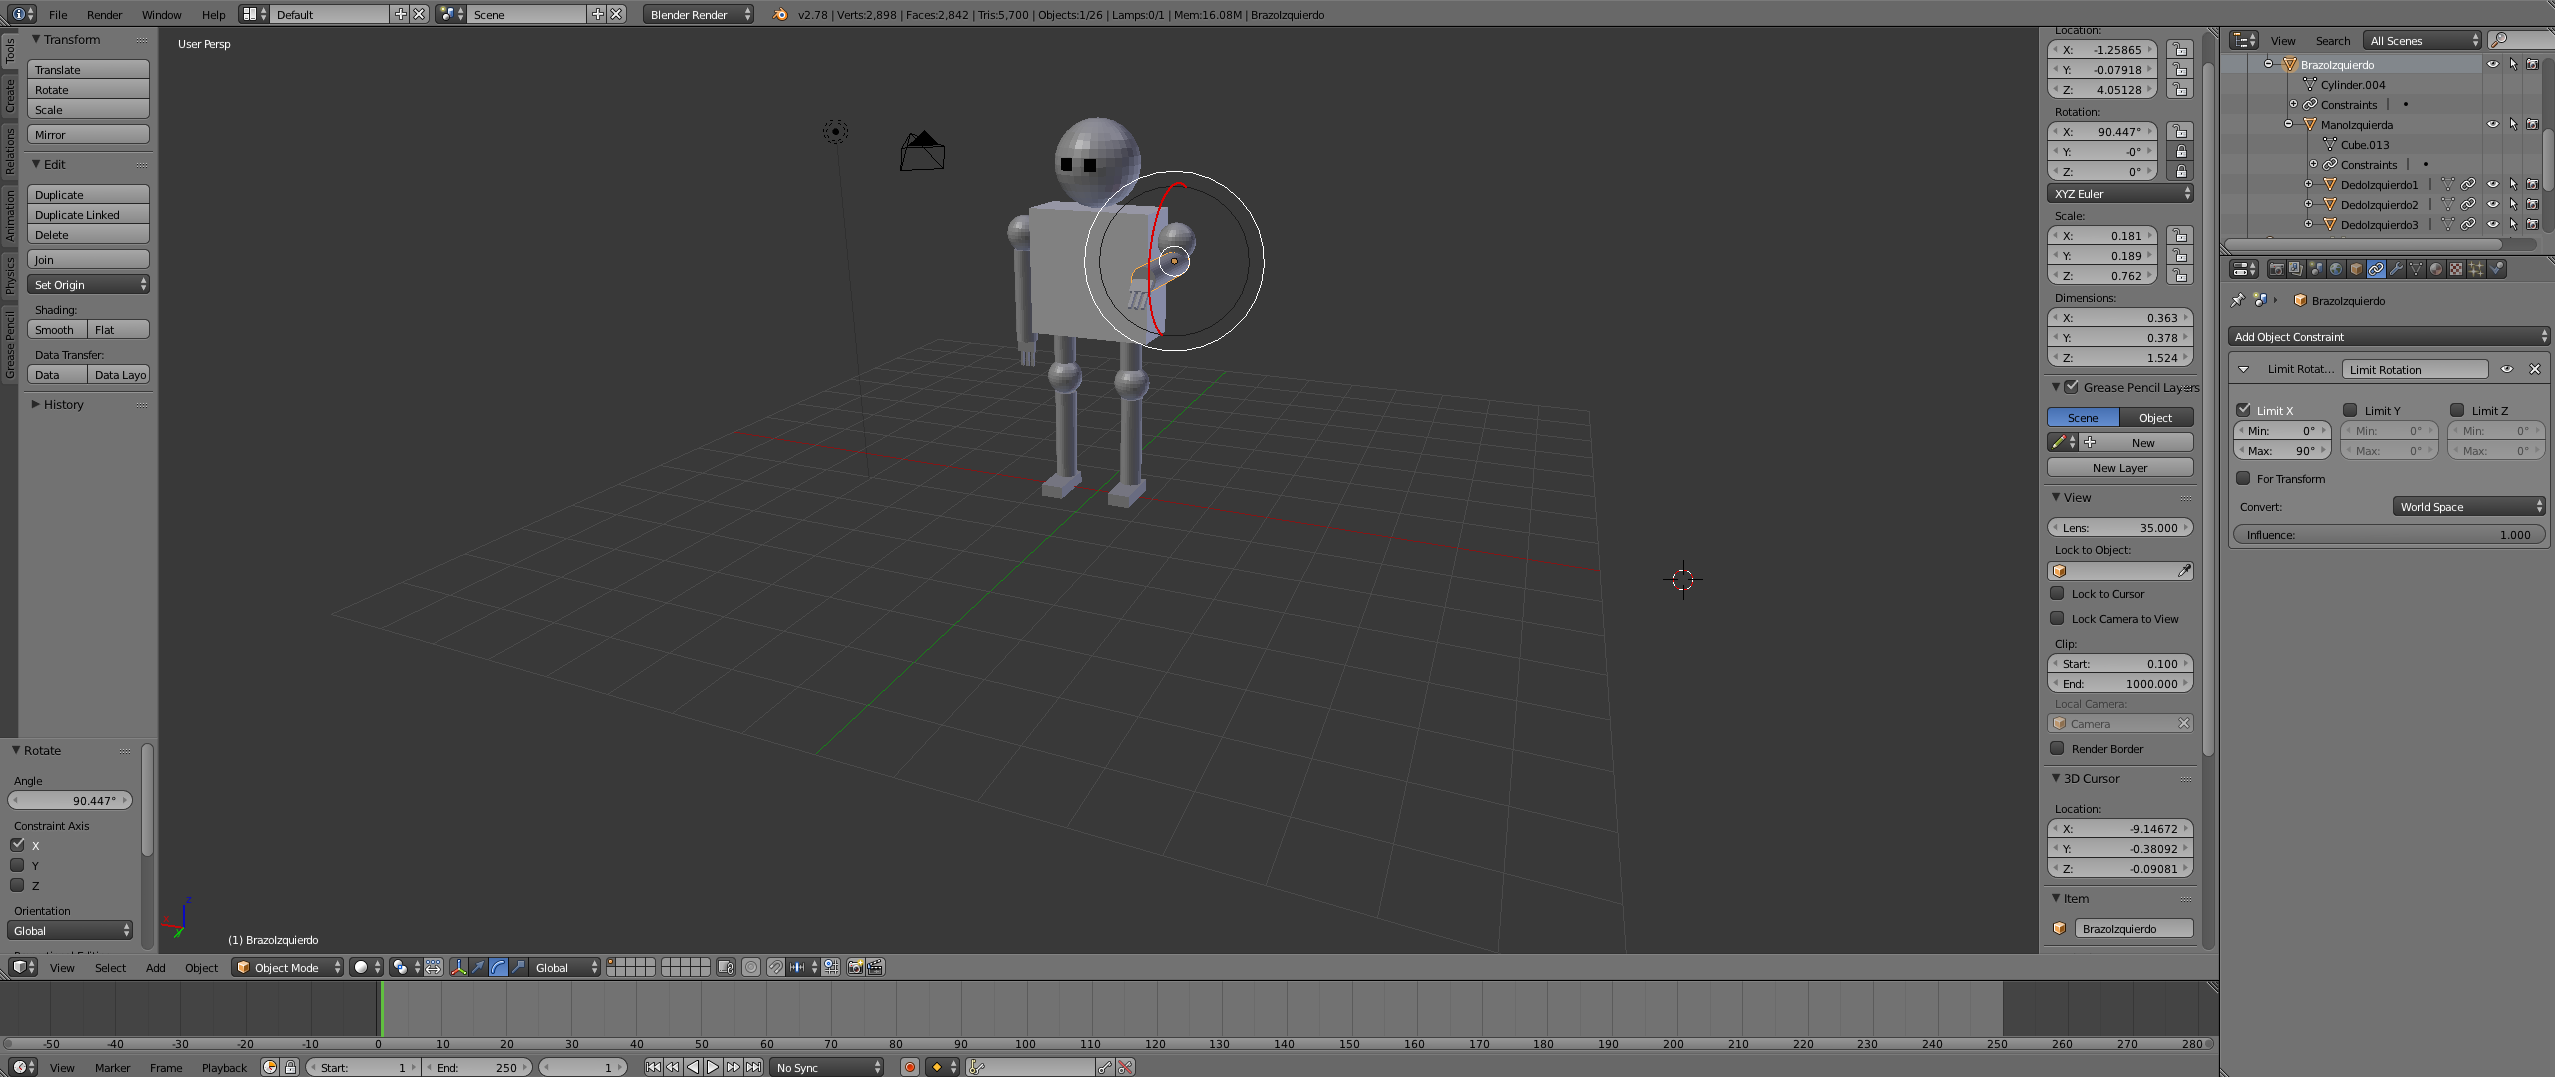
\includegraphics[width = 0.75\textwidth]{p2-img8}
 		\captionof{figure}{\label{fig:IPN}Buscando una imagen para crear el segundo contenedor.} 
	\end{center} 
\end{figure}


Con las imagenes de \textbf{MySQL} listadas, seleccionamos la primera para crear el segundo contenedor.\\

\begin{figure}[H]
	\begin{center}
 		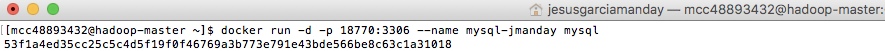
\includegraphics[width = 0.75\textwidth]{p2-img9}
 		\captionof{figure}{\label{fig:IPN}Creando el segundo contenedor.} 
	\end{center} 
\end{figure}

Comprobamos que se ha creado correctamente, y una vez verificado lo lanzamos y buscamos el servicio \textbf{MySQL}.\\

\begin{figure}[H]
	\begin{center}
 		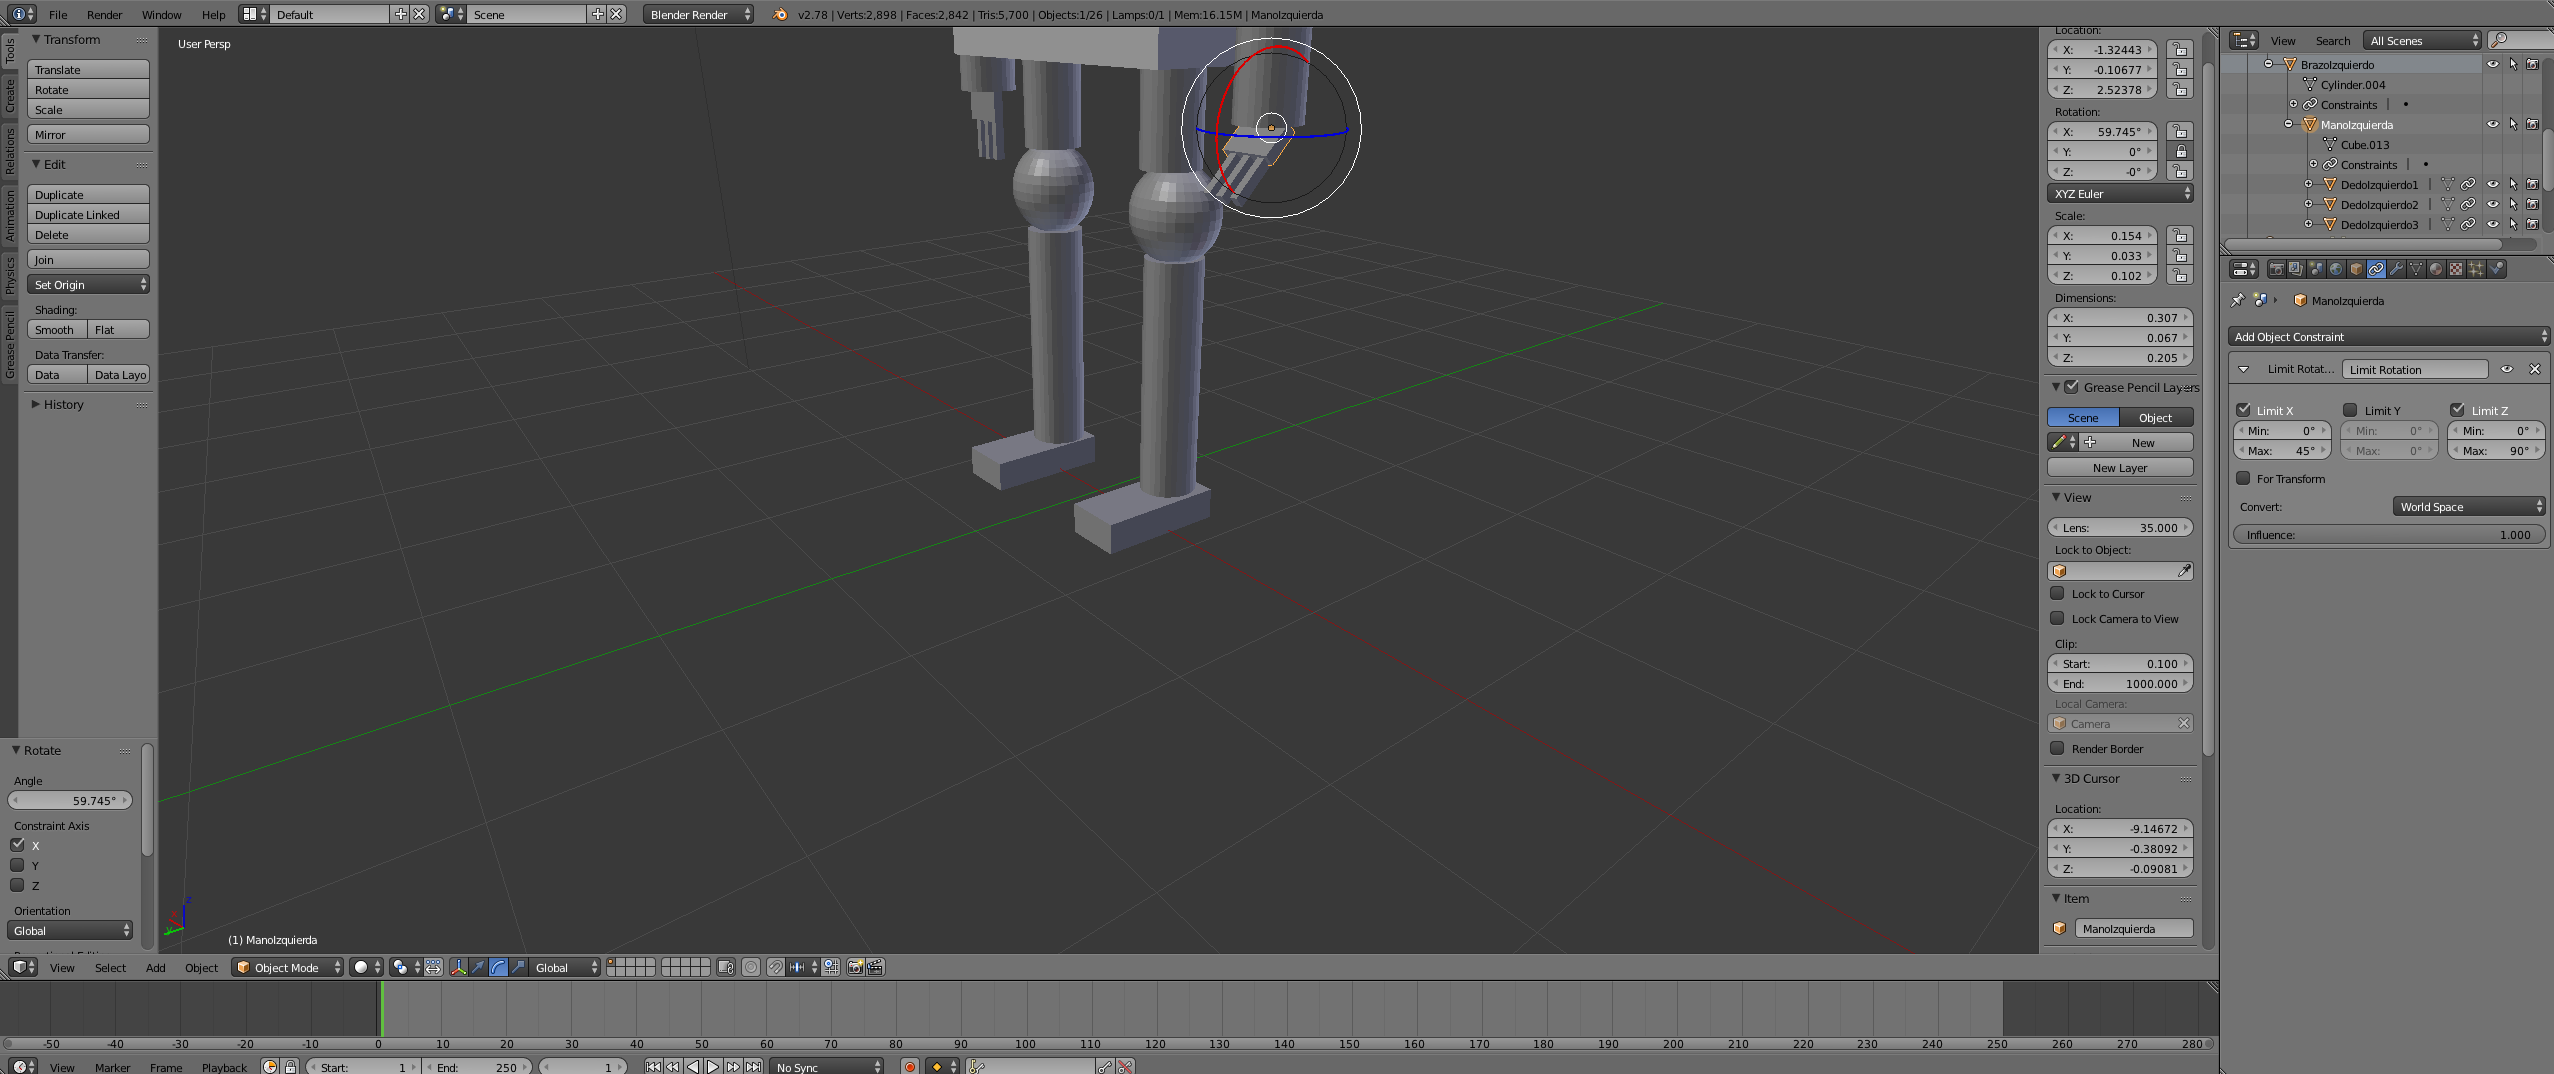
\includegraphics[width = 0.75\textwidth]{p2-img10}
 		\captionof{figure}{\label{fig:IPN}Lanzando el segundo contenedor.} 
	\end{center} 
\end{figure}

\begin{figure}[H]
	\begin{center}
 		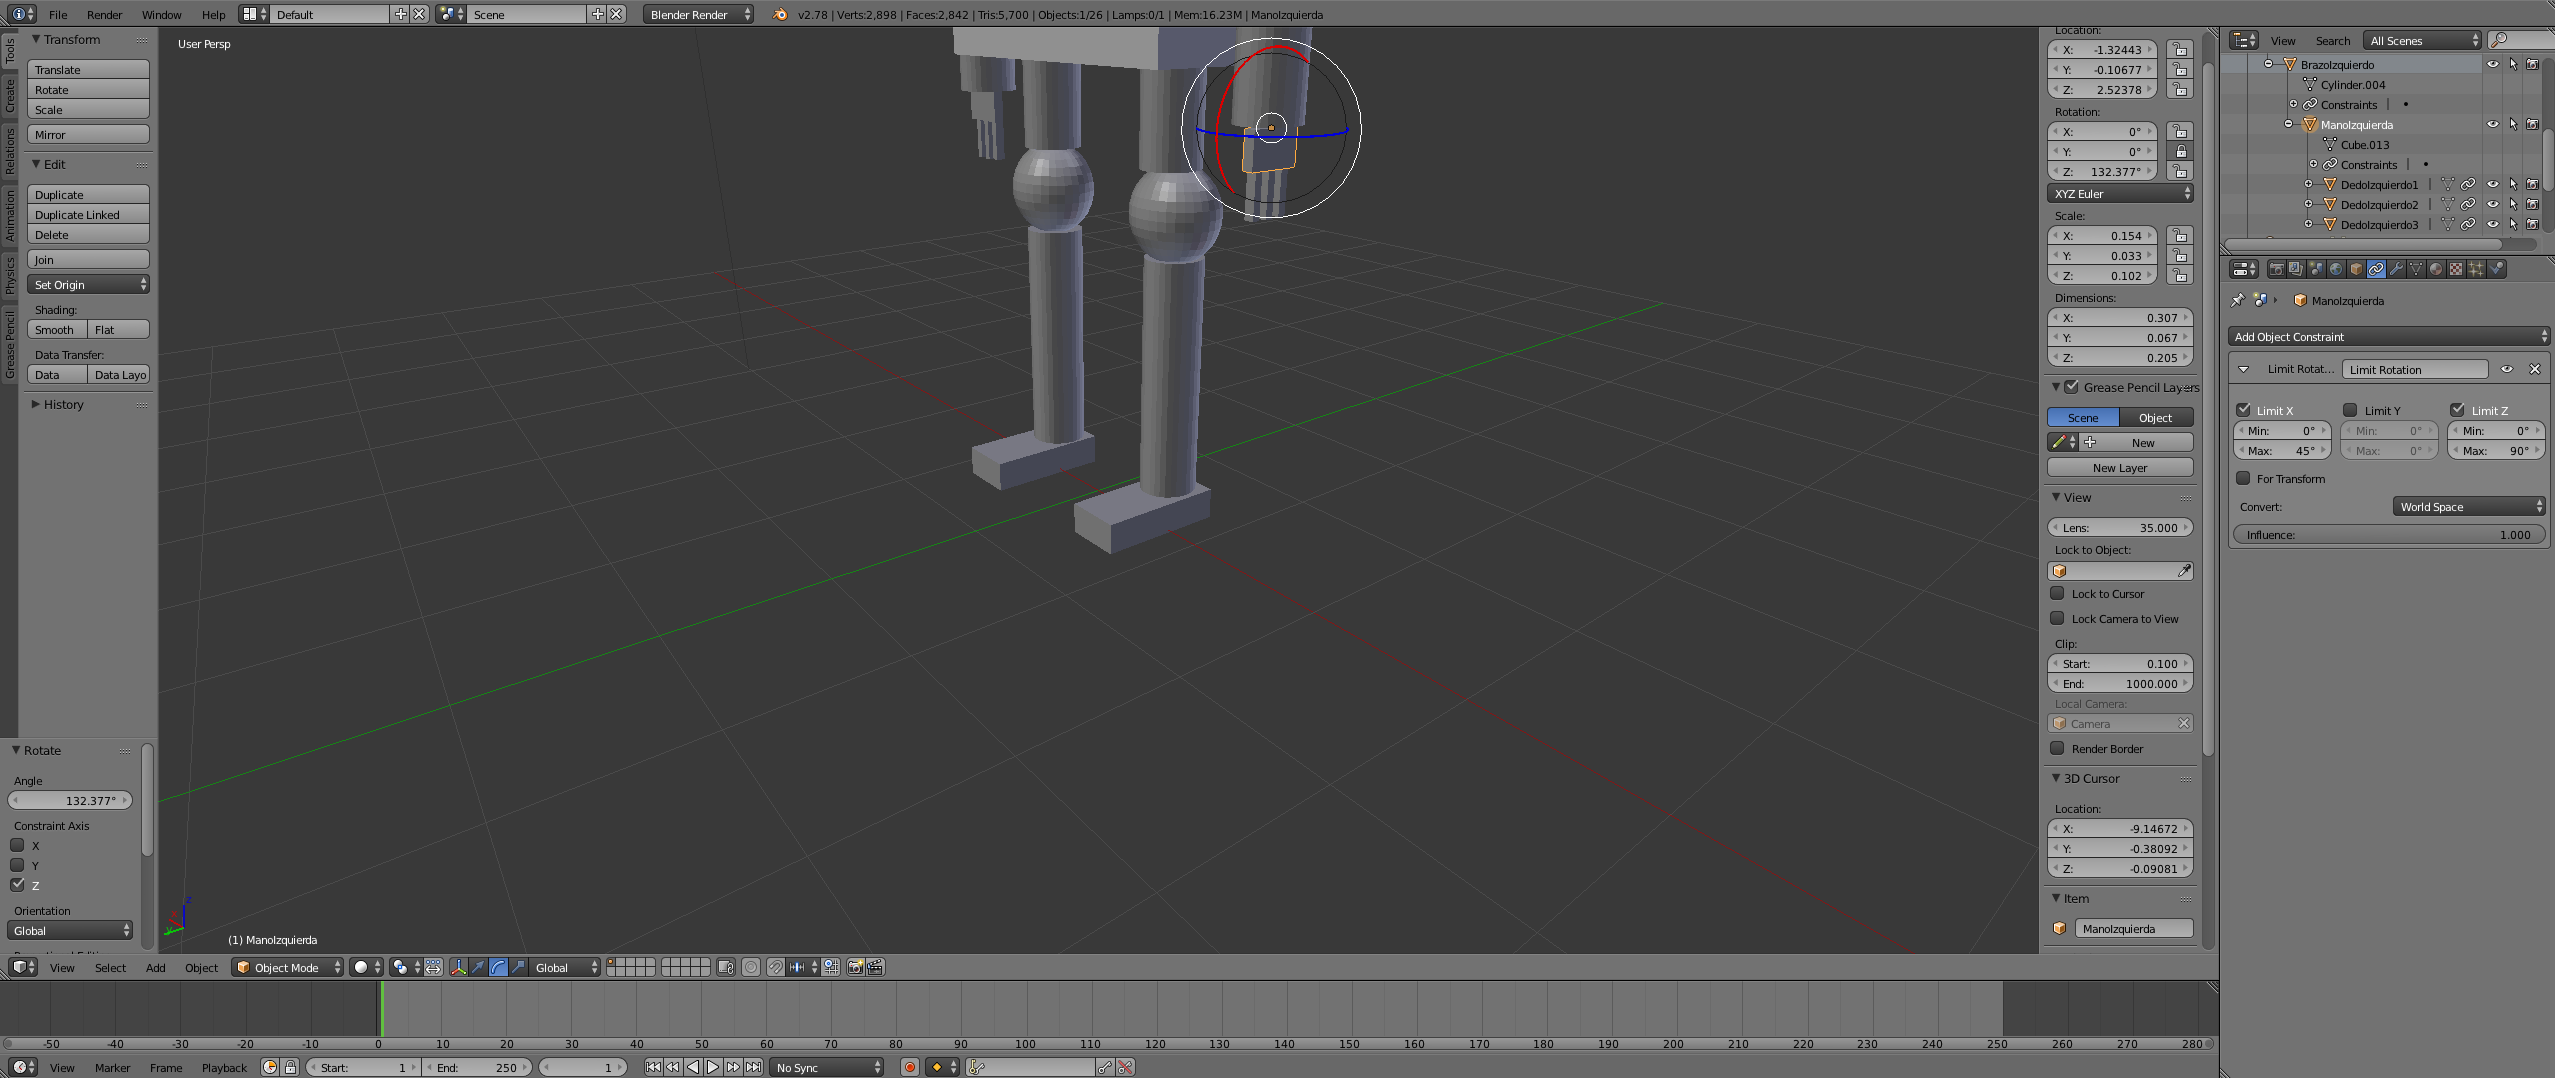
\includegraphics[width = 0.75\textwidth]{p2-img11}
 		\captionof{figure}{\label{fig:IPN}Comprobando que el segundo contenedor se ha creado.} 
	\end{center} 
\end{figure}

\begin{figure}[H]
	\begin{center}
 		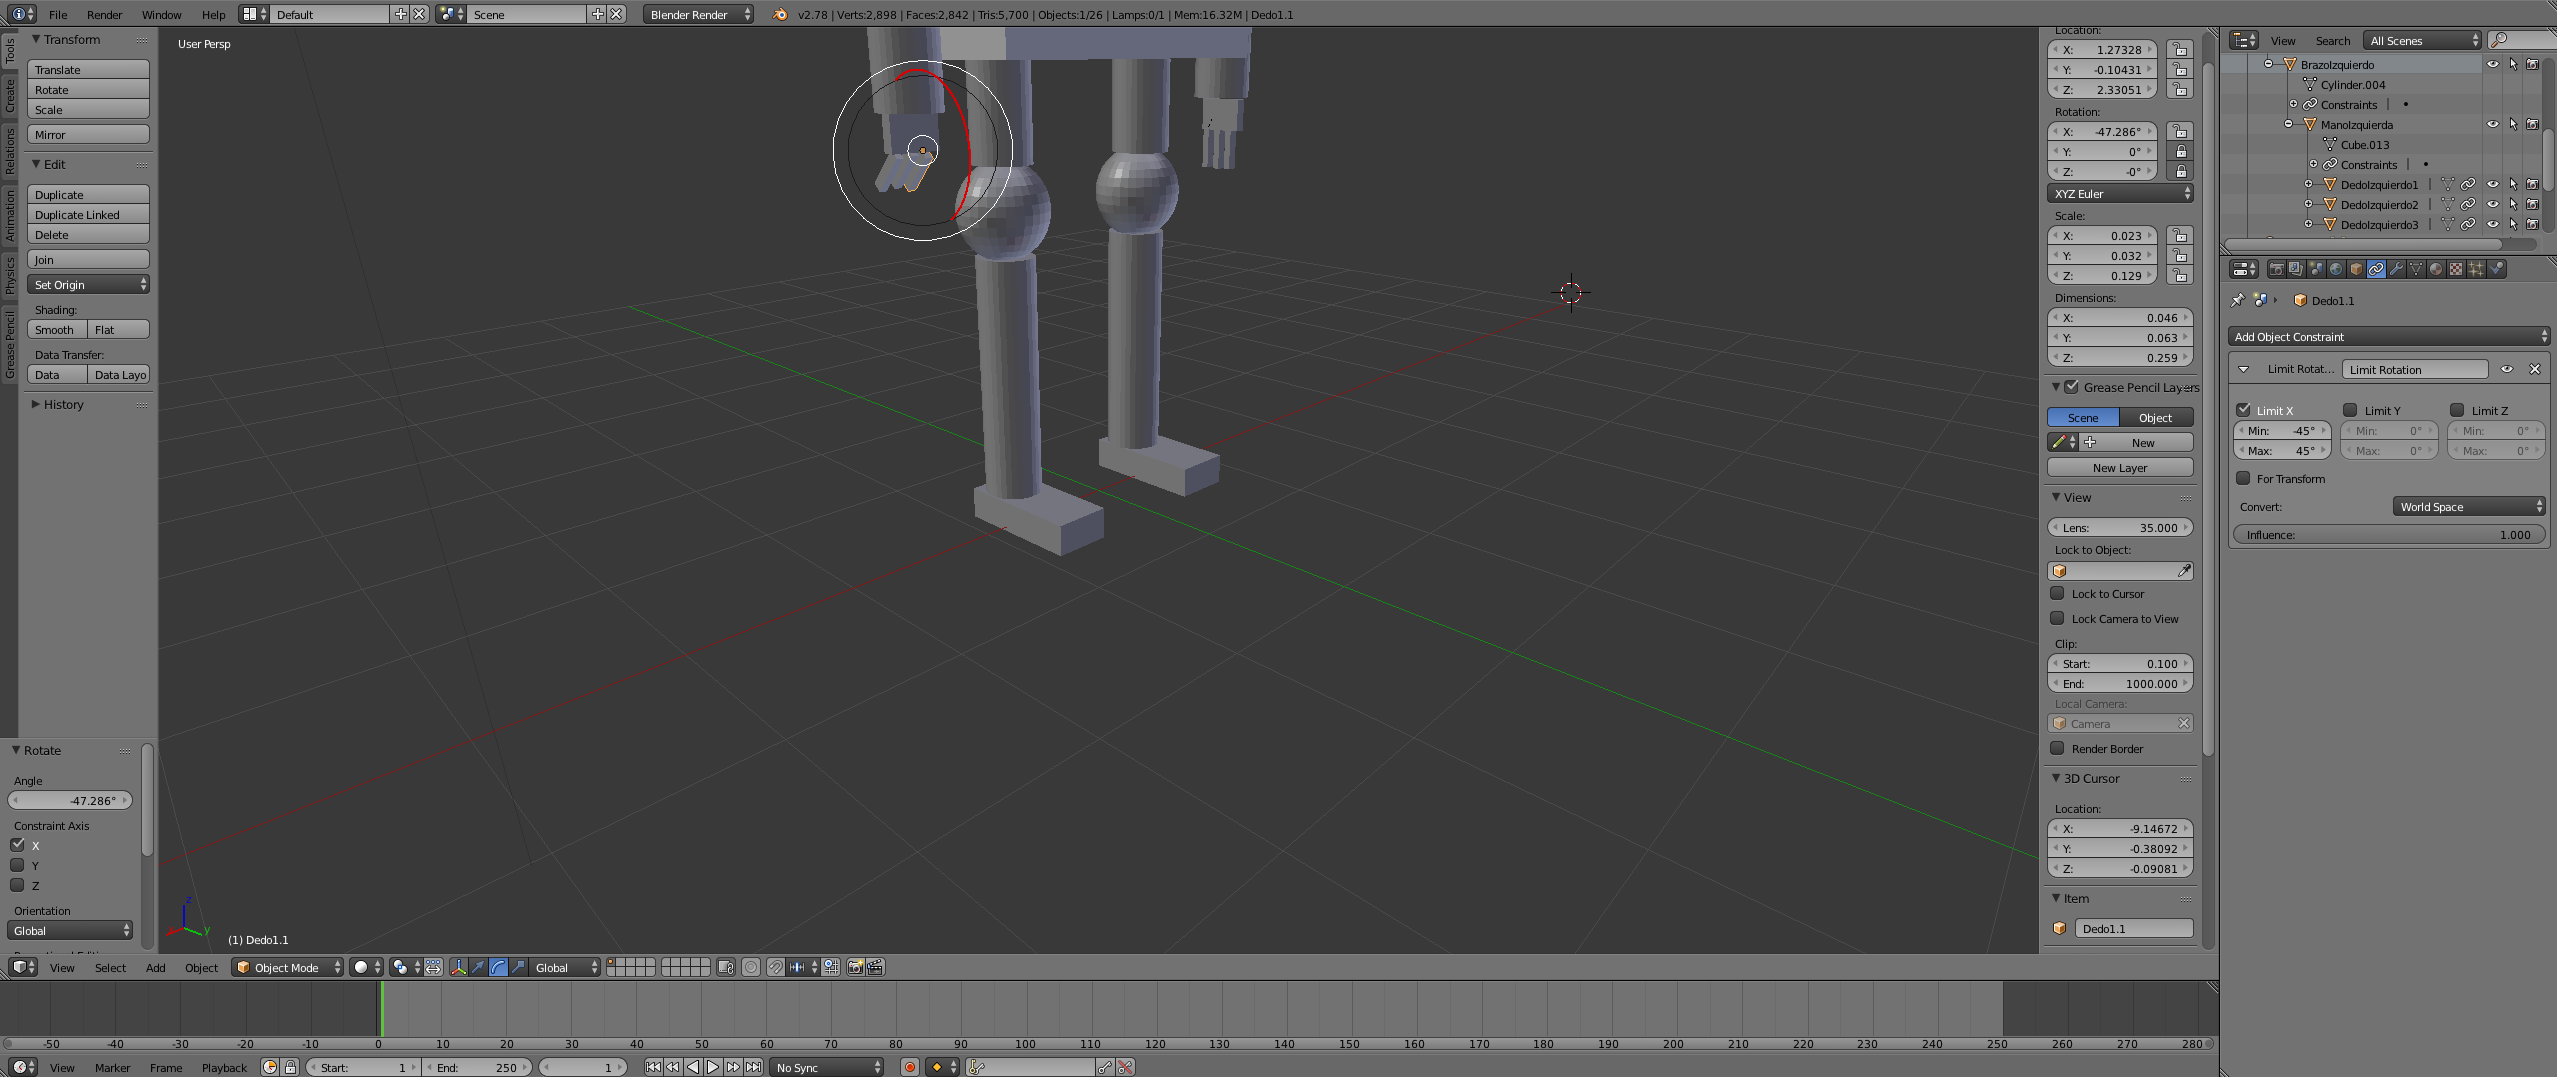
\includegraphics[width = 0.75\textwidth]{p2-img12}
 		\captionof{figure}{\label{fig:IPN}Comprobando que MySQL está instalado en el contenedor.} 
	\end{center} 
\end{figure}


\section{Configuración del servicio Web en docker.} 
Se ha tomado la configuración por defecto para el servicio Web instalado en el primer contenedor y para comprobar que funciona correctamente le lanzamos una petición a su página de inicio como se muestra en la siguiente figura.\\

\begin{figure}[H]
	\begin{center}
 		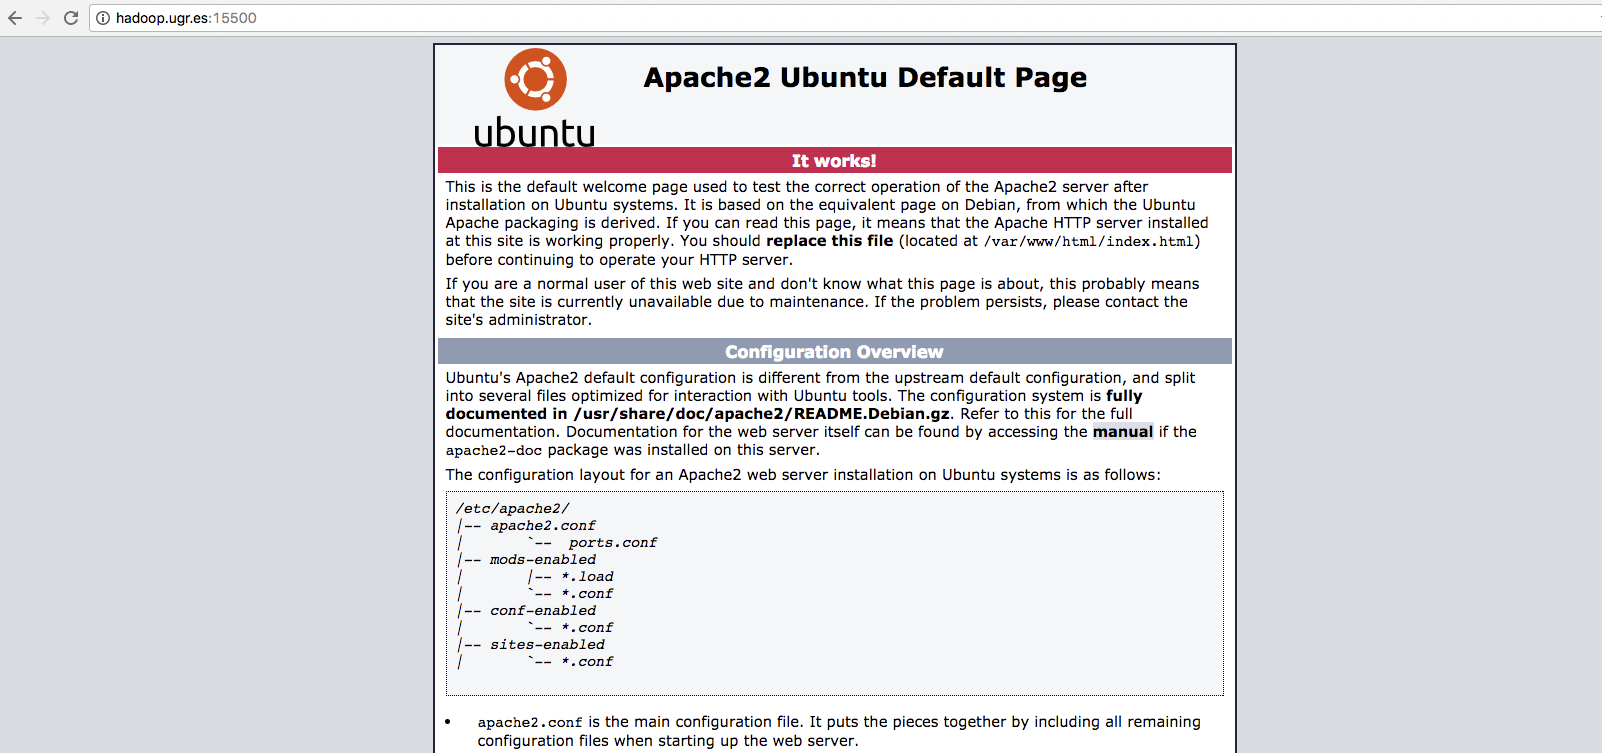
\includegraphics[width = 0.75\textwidth]{p2-img7}
 		\captionof{figure}{\label{fig:IPN}Configuración de Apache en docker.} 
	\end{center} 
\end{figure}


\section{Configuración del servicio de SGBD en docker.} 
Para este servicio instalado en el segundo contenedor se ha procedido a emplear la configuración por defecto al igual que en el apartado anterior con el servicio Web, por lo que el usuario de \textbf{MySQL} que se utilizará para conectarse a dicho servicio será el que viene por defecto (root). En la imagen de a continuación se puede ver como la configuración tomada es óptima. \\

\begin{figure}[H]
	\begin{center}
 		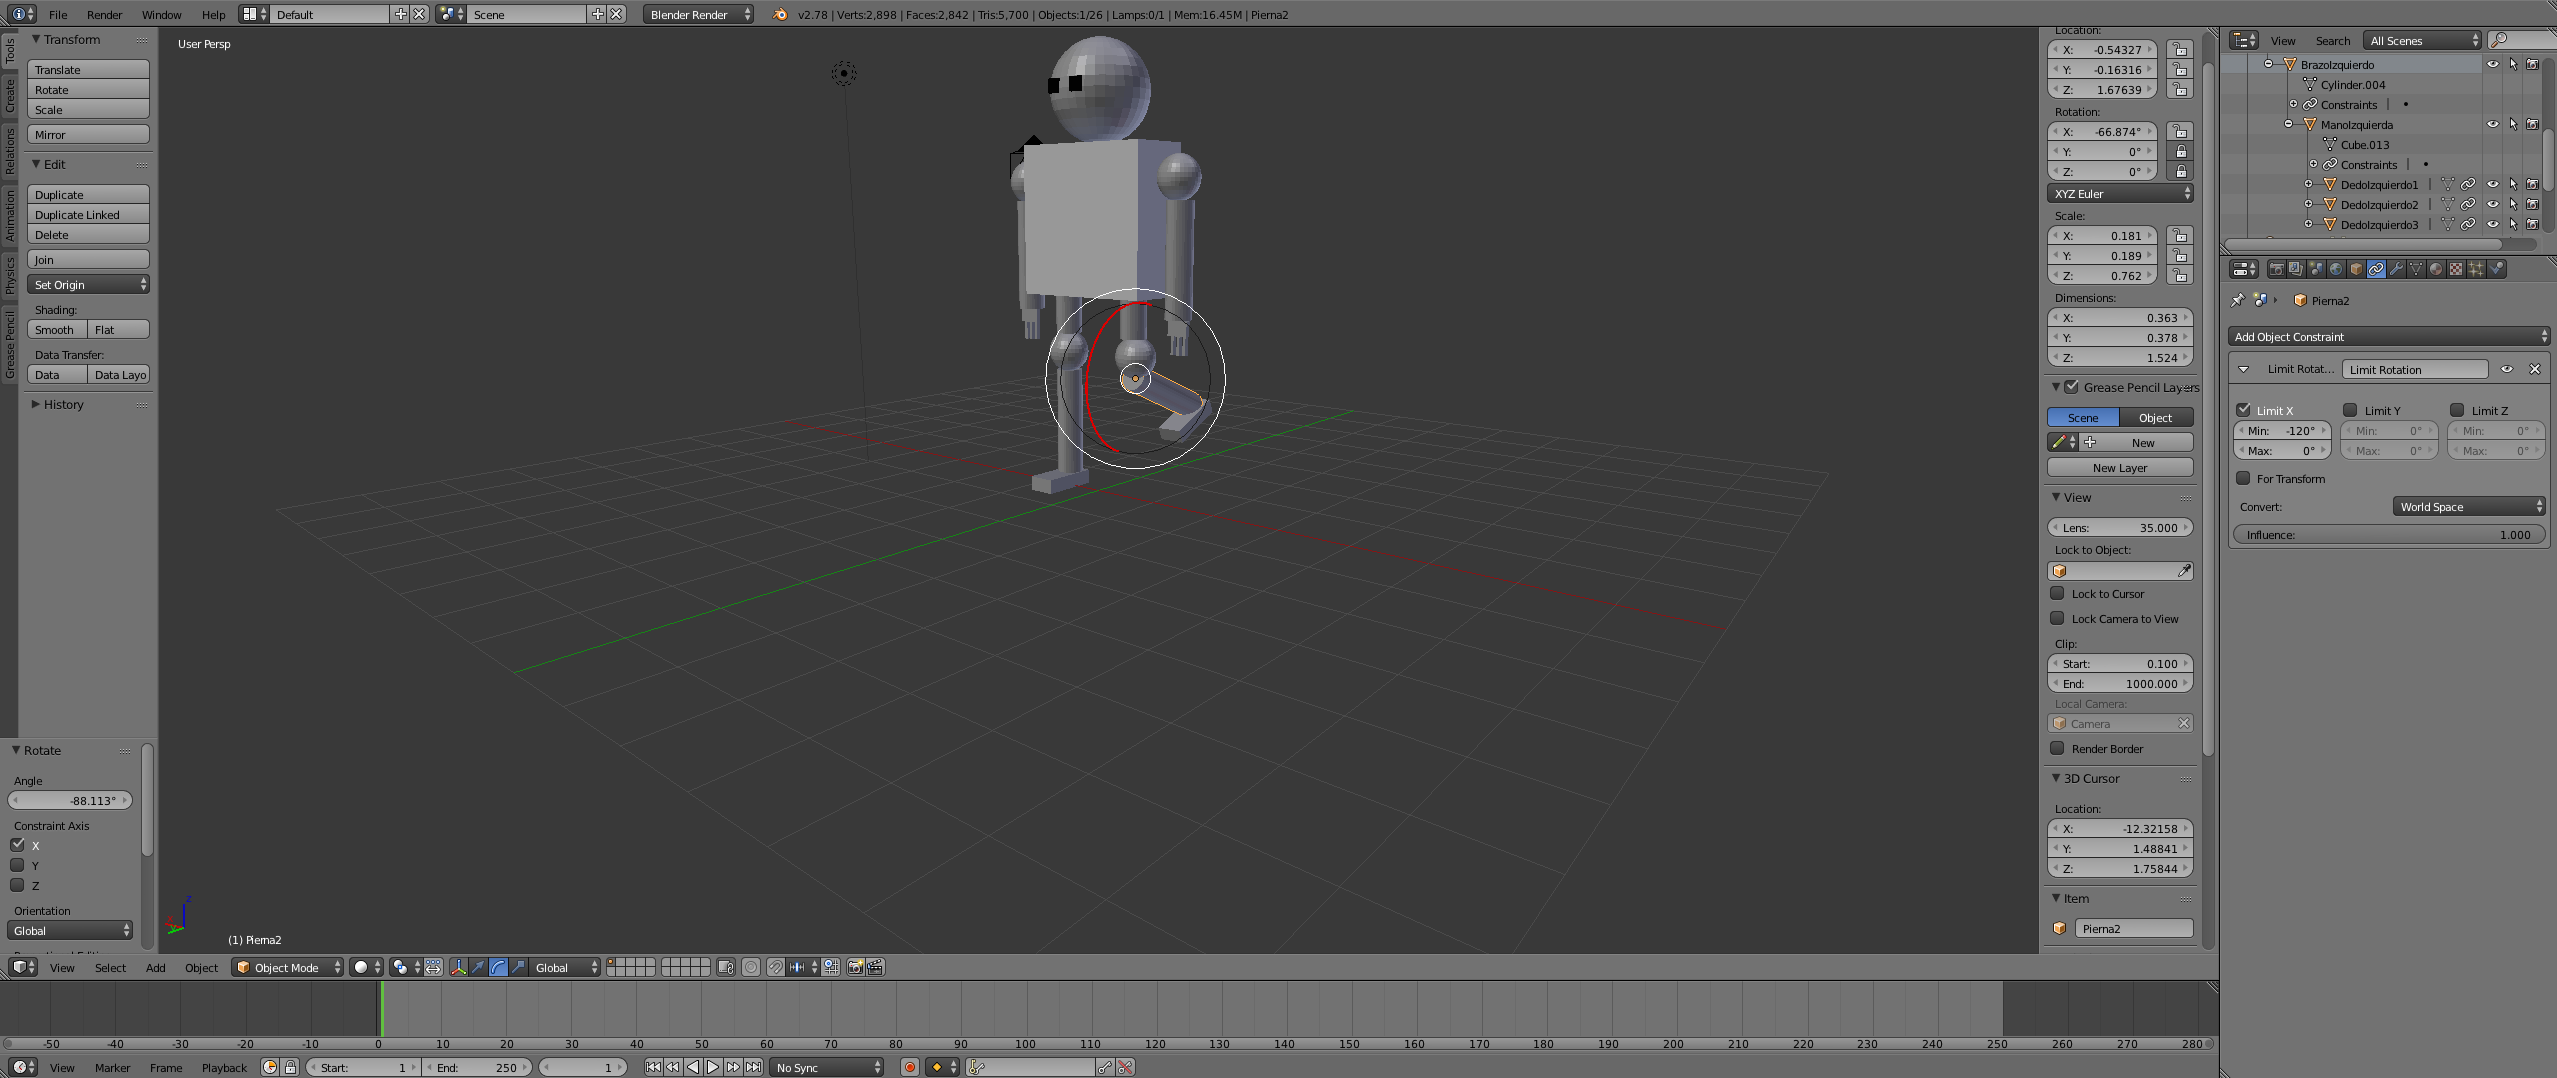
\includegraphics[width = 0.75\textwidth]{p2-img13}
 		\captionof{figure}{\label{fig:IPN}Configuración de MySQL en docker.} 
	\end{center} 
\end{figure}


\section{Descripción de la aplicación web. Objetivo, funcionalidad, arquitectura software, base de datos, tablas. Puedes utilizar la misma que en la Práctica 1 (IaaS). }
La aplicación que se va a estar ejecutando en el primer contenedor con el servicio Web \textbf{Apache} es una aplicación de gestión de usuarios que muestra una lista de los mismos y que permite las operaciones de insertar y eliminar usuarios de la base de datos que se encuentra en el segundo contenedor con el servicio de \textbf{MySQL}.\\

La arquitectura de la aplicación esta basada en microservicios, en este caso son dos los principales software  sobre los que se sustenta dicha aplicación (\textbf{Apache} y \textbf{MySQL}). Cada uno de los servicios mencionados residen en un contenedor diferente, comunicandose de forma remota entre ellos a través de protocolos de internet como http, icmp y tcp entre otros. En la siguiente imagen se puede apreciar la arquitectura en la que está basada la aplicación web.\\ \\

 \begin{figure}[H]
	\begin{center}
 		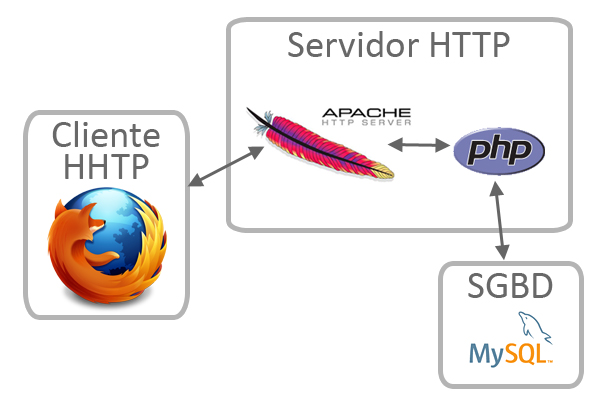
\includegraphics[width = 0.75\textwidth]{p2-img14}
 		\captionof{figure}{\label{fig:IPN}Arquitectura de la aplicación.} 
	\end{center} 
\end{figure}

En el primer contendor es donde se aloja el servidor Web de \textbf{Apache} y es por tanto donde se han definido los ficheros \textbf{php} que manejan las acciones realizadas por el usuario sobre la aplicación. Son tres los ficheros que se han implementado para el servidor los cuales residen en la dirección \textbf{/var/www/html} del mismo. El fichero por defecto que se ejecuta al acceder a la página inicial del servidor \url{http://hadoop.ugr.es:15500/} es el \textbf{index.php}, existen dos ficheros más que se encargan de cada una de las dos operaciones permitidas en la aplicación, la insercción de un nuevo usuario a través del fichero \textbf{insert\_user.php} y elminar a un usuario existente mediante el fichero \textbf{delete\_user.php}. En las siguientes imagenes se muestra la estructura y el contenido de dichos ficheros.\\ 

 \begin{figure}[H]
	\begin{center}
 		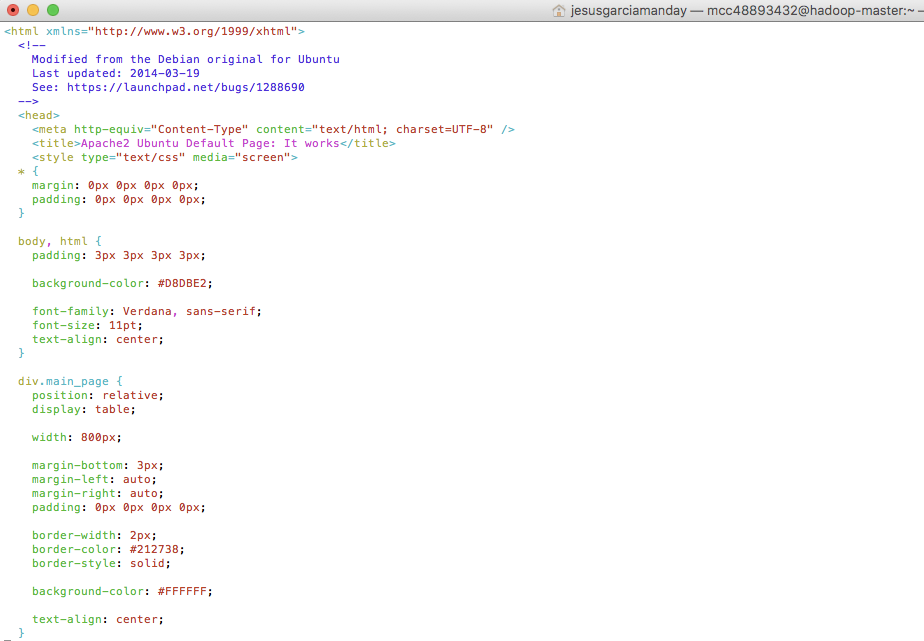
\includegraphics[width = 0.75\textwidth]{p2-img15}
 		\captionof{figure}{\label{fig:IPN}Fichero index.php (I).} 
	\end{center} 
\end{figure}

 \begin{figure}[H]
	\begin{center}
 		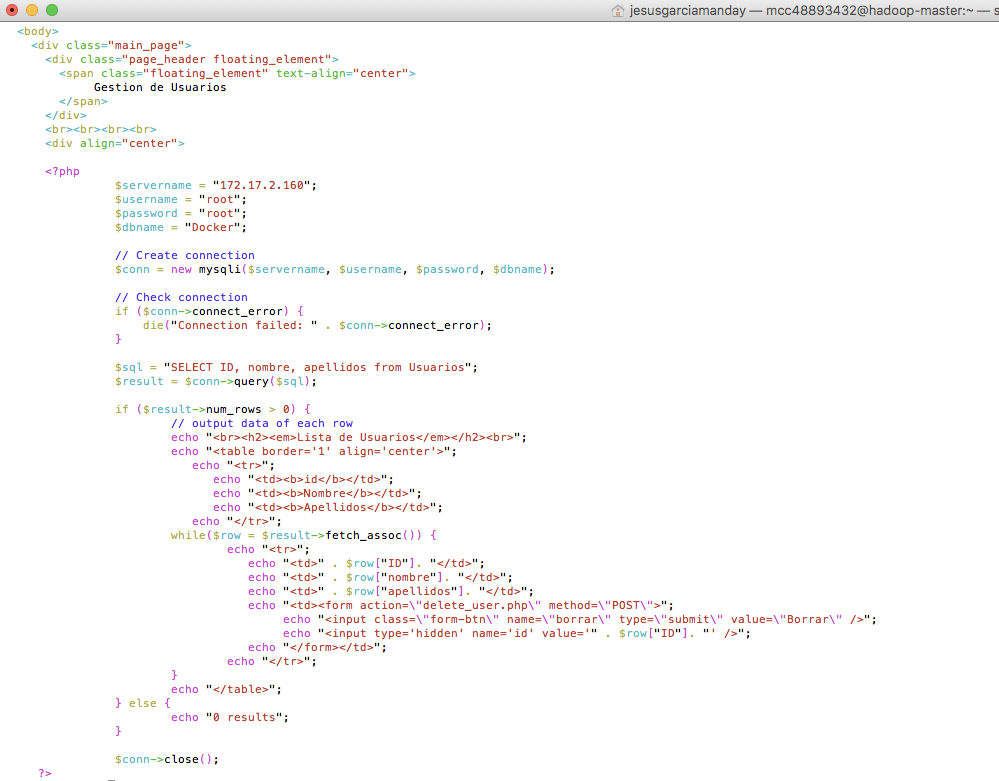
\includegraphics[width = 0.75\textwidth]{p2-img16}
 		\captionof{figure}{\label{fig:IPN}Fichero index.php (II).} 
	\end{center} 
\end{figure}

 \begin{figure}[H]
	\begin{center}
 		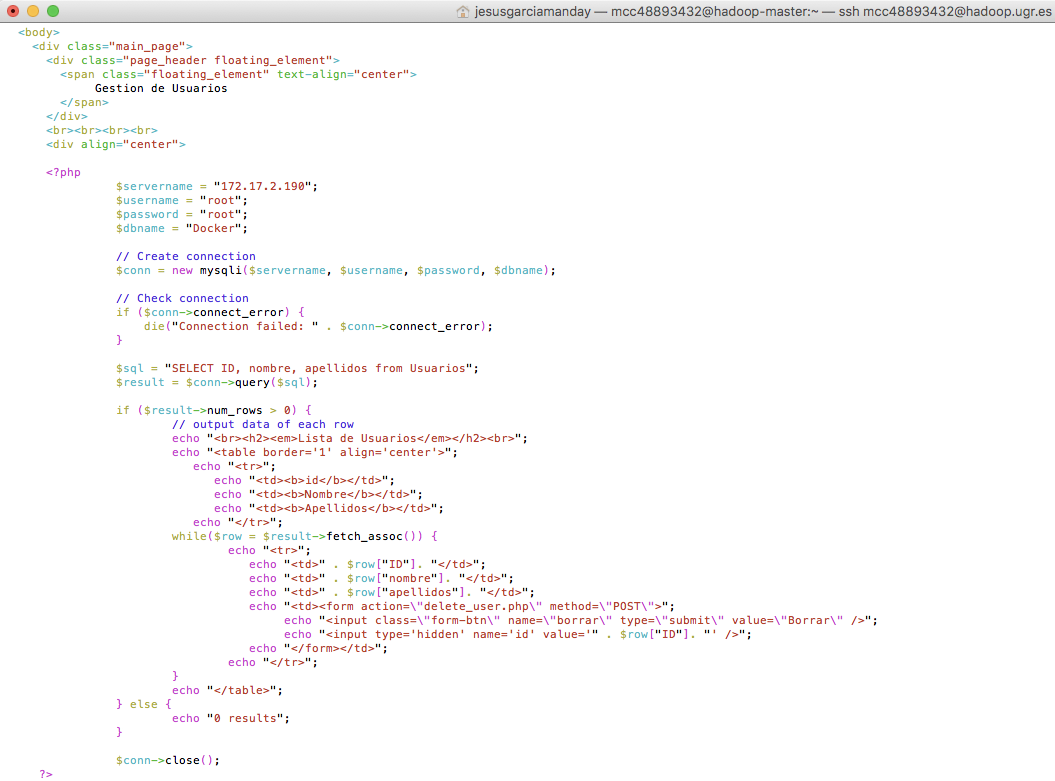
\includegraphics[width = 0.75\textwidth]{p2-img17}
 		\captionof{figure}{\label{fig:IPN}Fichero index.php (III).} 
	\end{center} 
\end{figure}

 \begin{figure}[H]
	\begin{center}
 		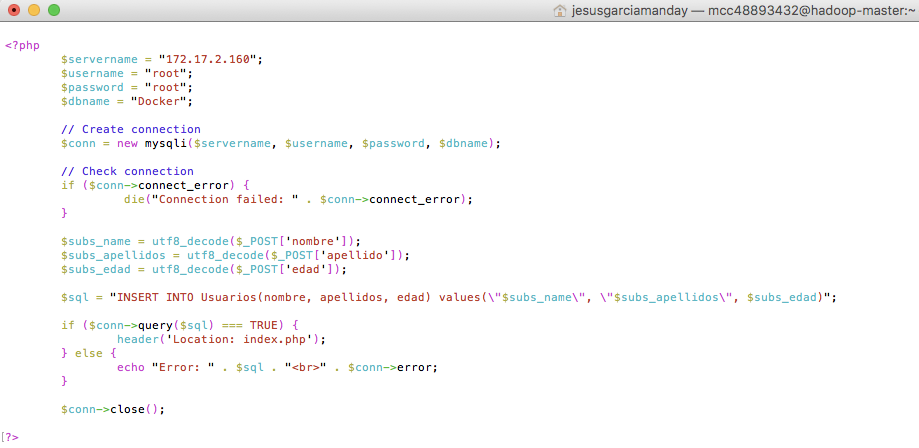
\includegraphics[width = 0.75\textwidth]{p2-img18}
 		\captionof{figure}{\label{fig:IPN}Fichero insert\_user.php .} 
	\end{center} 
\end{figure}

 \begin{figure}[H]
	\begin{center}
 		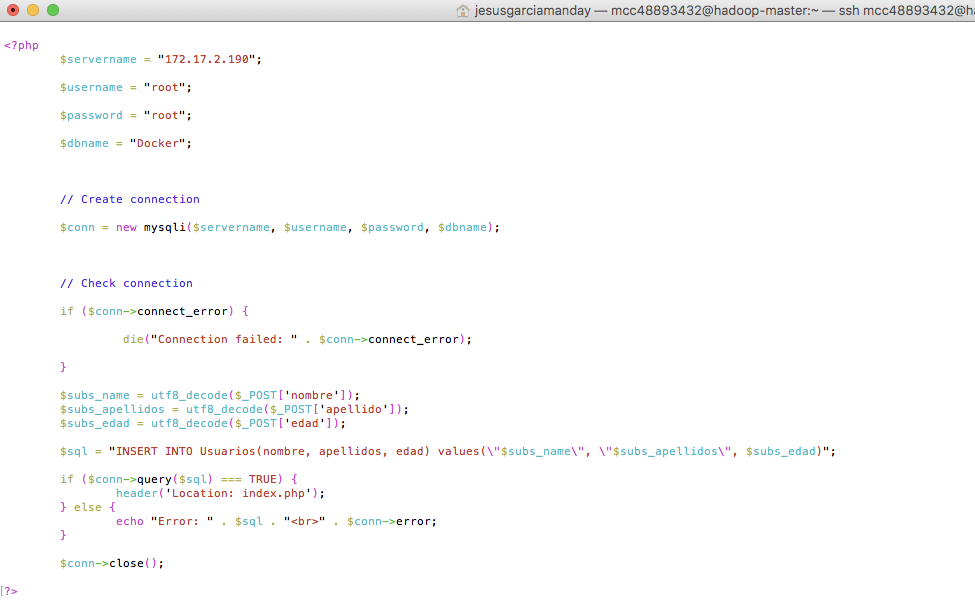
\includegraphics[width = 0.75\textwidth]{p2-img19}
 		\captionof{figure}{\label{fig:IPN}Fichero delete\_user.php .} 
	\end{center} 
\end{figure}

En el segundo contenedor es donde reside el SGBD \textbf{MySQL} y por lo tanto es donde se ha creado la base de datos correspondiente sobre la que trabaja la aplicación. En dicha base de datos se ha creado la tabla \textbf{Usuarios} la cual va a representar el modelo de datos para almacenar la información referente a los usuarios que se añadan o eliminen desde la aplicación. En las imagenes de a continuación se muestra la conexión hacia dicho contenedor así como el uso de la base de datos, la creación de la tabla y la insercción de algunos registros.\\

 \begin{figure}[H]
	\begin{center}
 		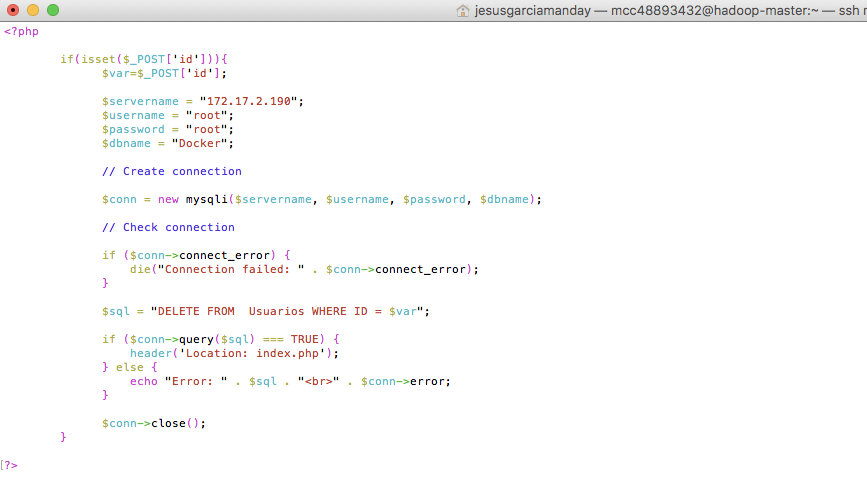
\includegraphics[width = 0.75\textwidth]{p2-img20}
 		\captionof{figure}{\label{fig:IPN}Creando tabla Usuarios en base de datos.} 
	\end{center} 
\end{figure} 

 \begin{figure}[H]
	\begin{center}
 		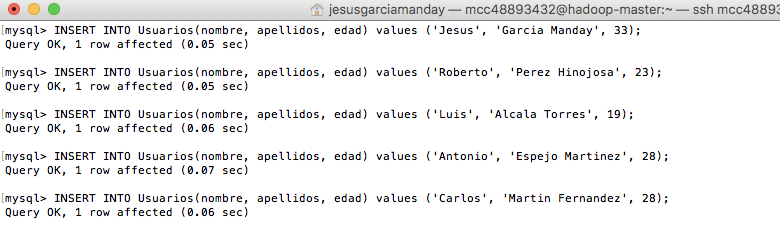
\includegraphics[width = 0.75\textwidth]{p2-img21}
 		\captionof{figure}{\label{fig:IPN}Insertando registros en la base de datos.} 
	\end{center} 
\end{figure} 


El resultado final de la aplicación lo podemos ver ejecutando desde el navegador de otra máquina cualquiera la dirección \url{http://hadoop.ugr.es:15500/} como se aprecia en la imagen de abajo.\\

 \begin{figure}[H]
	\begin{center}
 		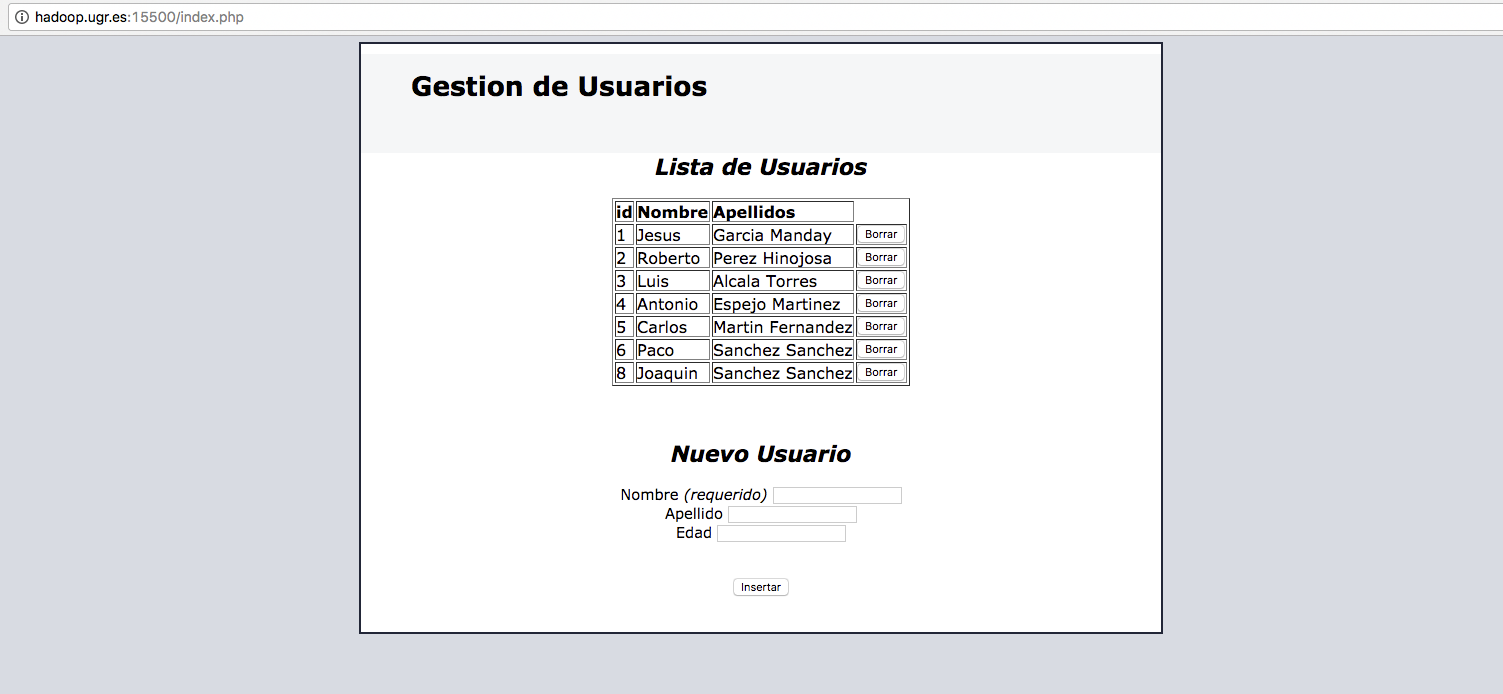
\includegraphics[width = 0.75\textwidth]{p2-img22}
 		\captionof{figure}{\label{fig:IPN}Aplicación web.} 
	\end{center} 
\end{figure}


\section{Análisis de la funcionalidad de los contenedores replicados.} 
Existe una funcionalidad a partir de la versión \textbf{1.12} de \textbf{Docker} que permite crear un clúster formado por varios Docker Hosts llamada \textbf{Swarm Mode}. \\

En un clúster de Swarm existen dos tipos de nodo, \textbf{Manager} y \textbf{Worker}. Los nodos \textbf{Manager} son los encargados de gestionar el clúster. Entre todos los Manager se elige automáticamente un líder que será el encargado de mantener el estado del clúster.\\

Los \textbf{Manager} también son los encargados de distribuir las tareas o task (unidades básicas de trabajo) entre todos los nodos \textbf{Worker}, los cuales reciben estas tareas y las ejecutan. Los nodos Manager por defecto también actúan como nodos Worker aunque se su configuración se puede cambiar para que solo asuma tareas de Manager. En la siguiente imagen se puede ver el esquema de esta funcionalidad de \textbf{Docker}.\\

 \begin{figure}[H]
	\begin{center}
 		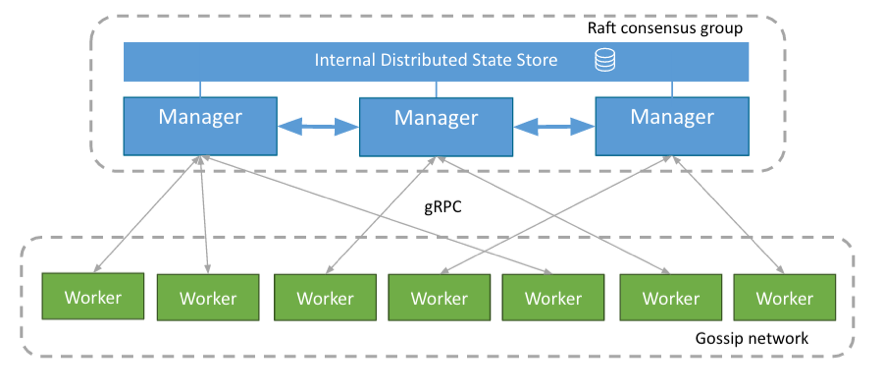
\includegraphics[width = 0.75\textwidth]{p2-img31}
 		\captionof{figure}{\label{fig:IPN}Estructura Swarm Mode.} 
	\end{center} 
\end{figure}

\textbf{Swarm} incluye además nuevas funcionalidades como \textbf{escalado, balanceo de carga} y \textbf{rolling updates}. Estas 
utilidades serán empleadas con los dos contenedores creados anteriormente, ya que la idea es crear un clúster de contenedores donde exista dos nodos \textbf{Manager} (uno para el servicio Web y otro para la base de datos), y un conjunto de nodos \textbf{Worker} reunidos en dos grupos, uno que lo gestionará el nodo \textbf{Manager} del servicio Web, y otro que lo administrará el nodo \textbf{Manager} de la base de datos. En cada uno de los grupos se replicará el servicio del servicio de un contenedor principal, es decir, en los nodos \textbf{Worker} que sean gestionados por el nodo \textbf{Manager} del servicio Web se replicará todo lo referente a la aplicación y servicios instalados (ficheros php, Apache, etc), mientras que en los nodos \textbf{Worker} gestionados por el nodo \textbf{Manager} de la base de datos se replicará esta misma sobre todos los nodos, de manera que la información (tablas, registros, etc) quedará replicada en cada nodo. \\

Al hacer esto el proyecto gana en robustez y rapidez, ya que las funcionalidades de escalado y balanceo de carga van a permitir que los servicios sigan activos aunque algún nodo haya caído por cualquier problema, y que no exista sobrecarga a un sólo nodo y la carga de trabajo o tareas sea repartida entre los diferentes nodos del clúster.\\

\section{Configuración de OwnCloud en docker.} 
En este punto se va a proceder a configurar el servicio \textbf{ownCloud} en un contenedor \textbf{Docker}. De este manera se consigue tener dicha aplicación de un modo más aislado y portable, evitando también el instalarla directamente sobre la máquina.\\

Lo primero que haremos será buscar si existe alguna imagen en \textbf{Docker} con dicho servicio, para ello volvemos a usar el comando \textbf{docker hub}.\\

 \begin{figure}[H]
	\begin{center}
 		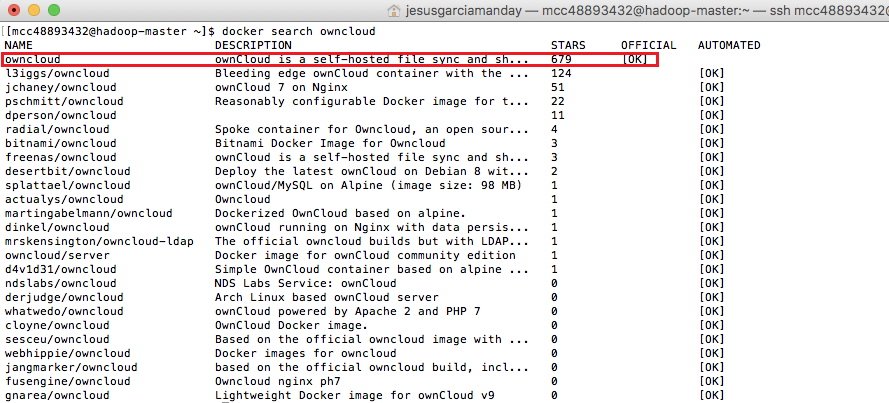
\includegraphics[width = 0.75\textwidth]{p2-img23}
 		\captionof{figure}{\label{fig:IPN}Buscando imagen en Docker.} 
	\end{center} 
\end{figure}

Como se aprecia en la anterior figura, existe una imagen en \textbf{Docker} con el servicio \textbf{ownCloud}. Es esta la imagen que vamos a utilizar para crear y lanzar un contenedor con dicho servicio. Antes de lanzar el contenedor con \textbf{OwnCloud} vamos a lanzar otro que tenga el servicio de \textbf{PostgreSQL} del que habiendo buscado en el hub de \textbf{Docker} se ha podido ver que existe una imagen oficial con dicho servicio.\\

 \begin{figure}[H]
	\begin{center}
 		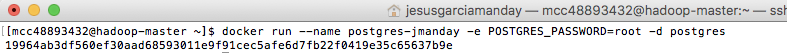
\includegraphics[width = 0.75\textwidth]{p2-img24}
 		\captionof{figure}{\label{fig:IPN}Lanzando contendor con PostgreSQL en Docker.} 
	\end{center} 
\end{figure}

Con el contenedor de \textbf{PostgreSQL} lanzado, lo siguiente es lanzar el contenedor de \textbf{ownCloud} al cual se le enlazará el host (contenedor) con la base de datos creada anteriormente. \\ 

  \begin{figure}[H]
	\begin{center}
 		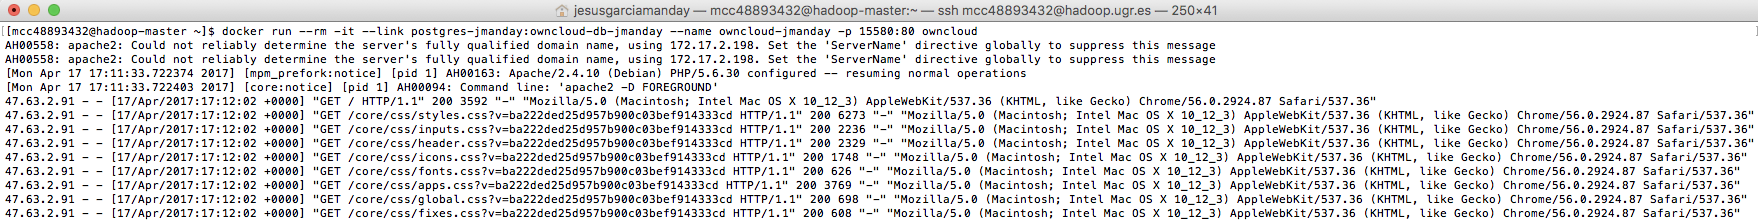
\includegraphics[width = 0.75\textwidth]{p2-img25}
 		\captionof{figure}{\label{fig:IPN}Lanzando contendor con ownCloud en Docker.} 
	\end{center} 
\end{figure}

  \begin{figure}[H]
	\begin{center}
 		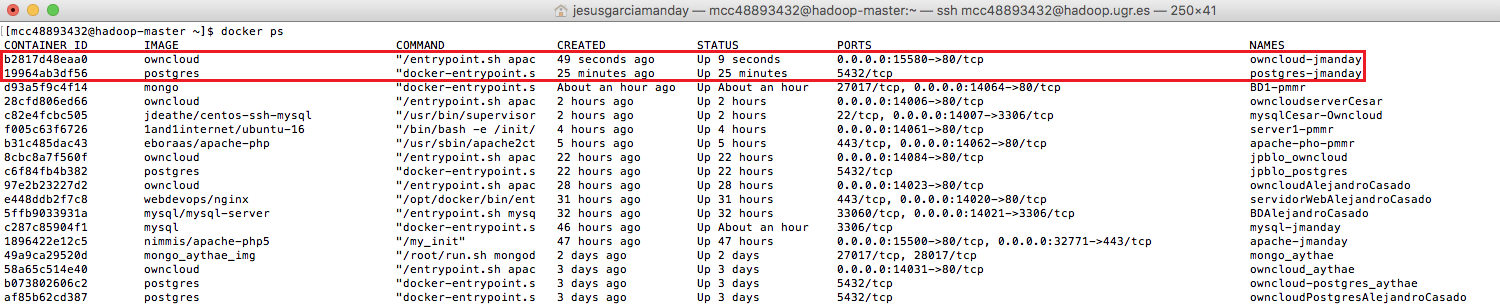
\includegraphics[width = 0.75\textwidth]{p2-img26}
 		\captionof{figure}{\label{fig:IPN}Comprobando que ambos contenedores se han lanzado correctamente.} 
	\end{center} 
\end{figure}

  \begin{figure}[H]
	\begin{center}
 		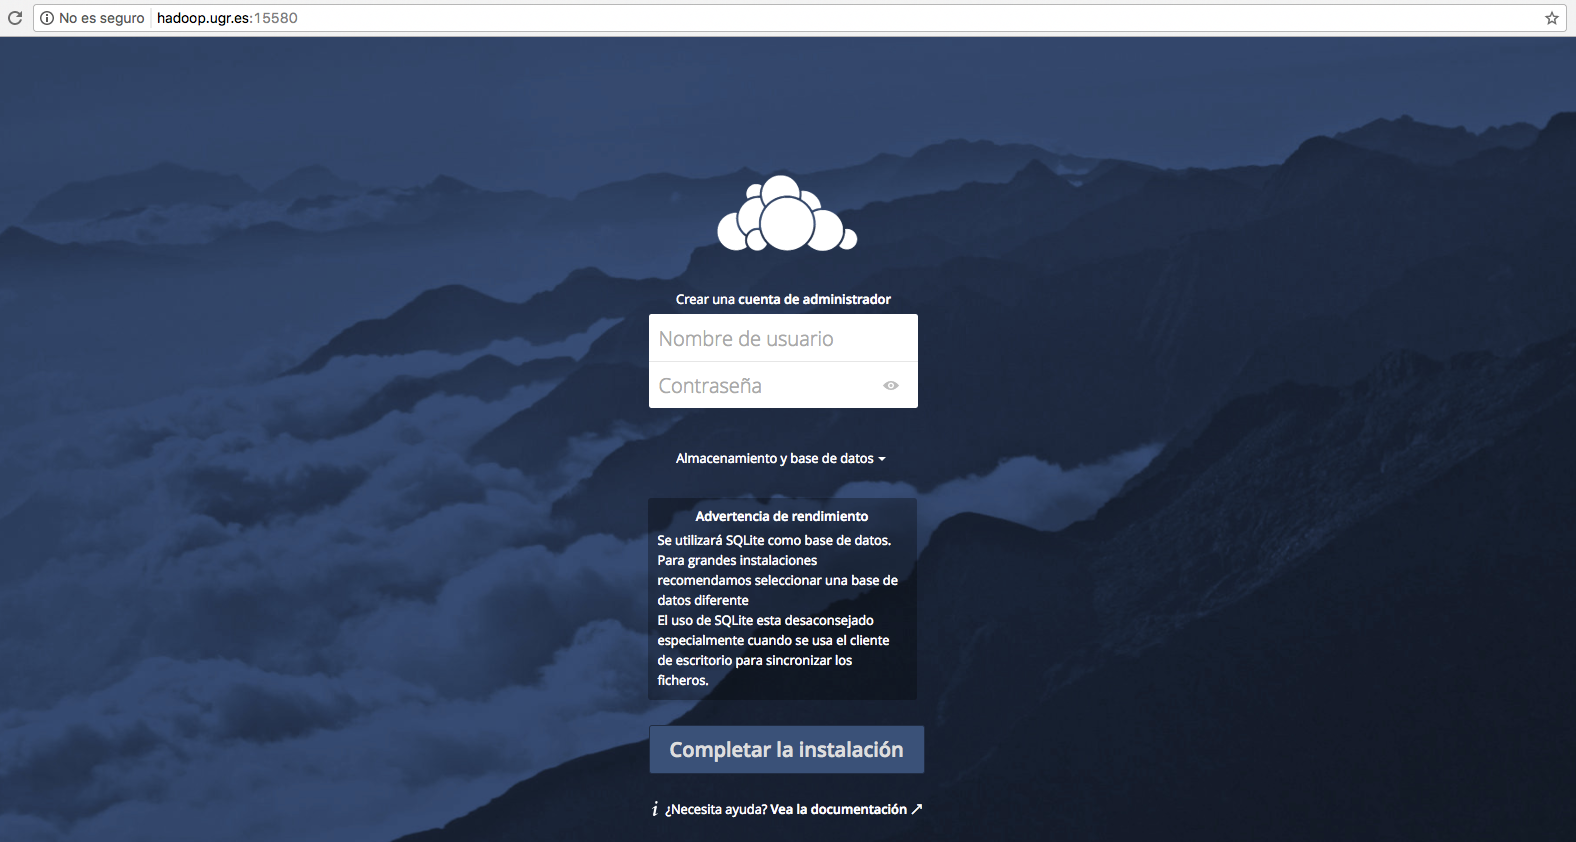
\includegraphics[width = 0.75\textwidth]{p2-img27}
 		\captionof{figure}{\label{fig:IPN}Comprobando que se esta ejecutando la aplicación.} 
	\end{center} 
\end{figure}

Una vez realizados los pasos anteriores, se puede comprobar con las imagenes como la configuración del servicio \textbf{ownCloud} se ha realizado correctamente y su funcionamiento es el deseado. \\

  \begin{figure}[H]
	\begin{center}
 		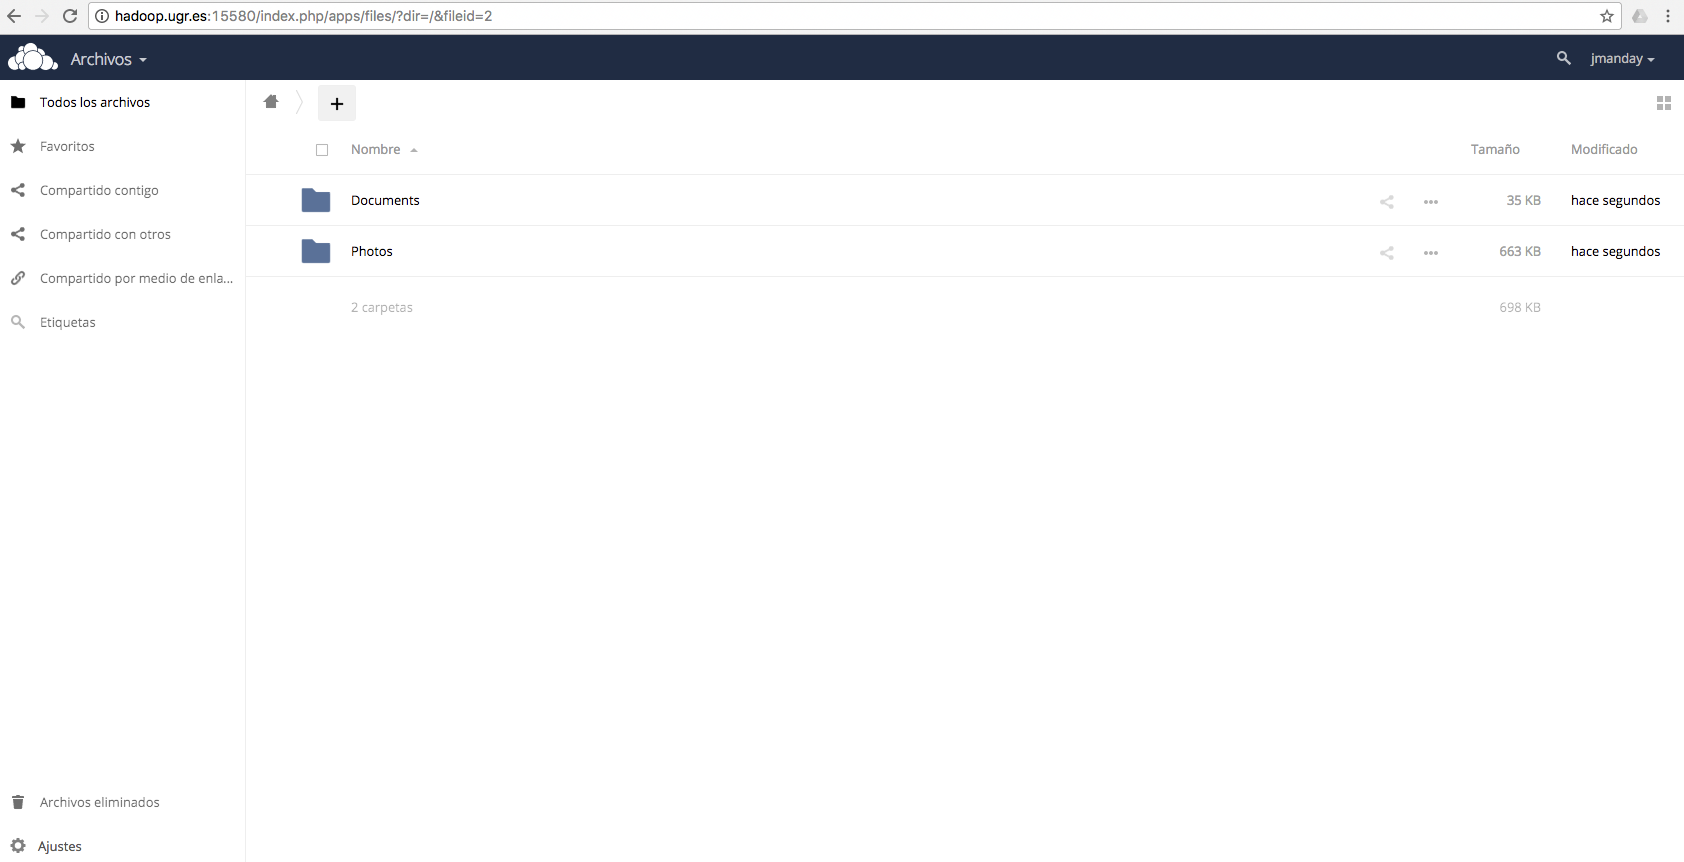
\includegraphics[width = 0.75\textwidth]{p2-img28}
 		\captionof{figure}{\label{fig:IPN}Probando ownCloud (I).} 
	\end{center} 
\end{figure}

  \begin{figure}[H]
	\begin{center}
 		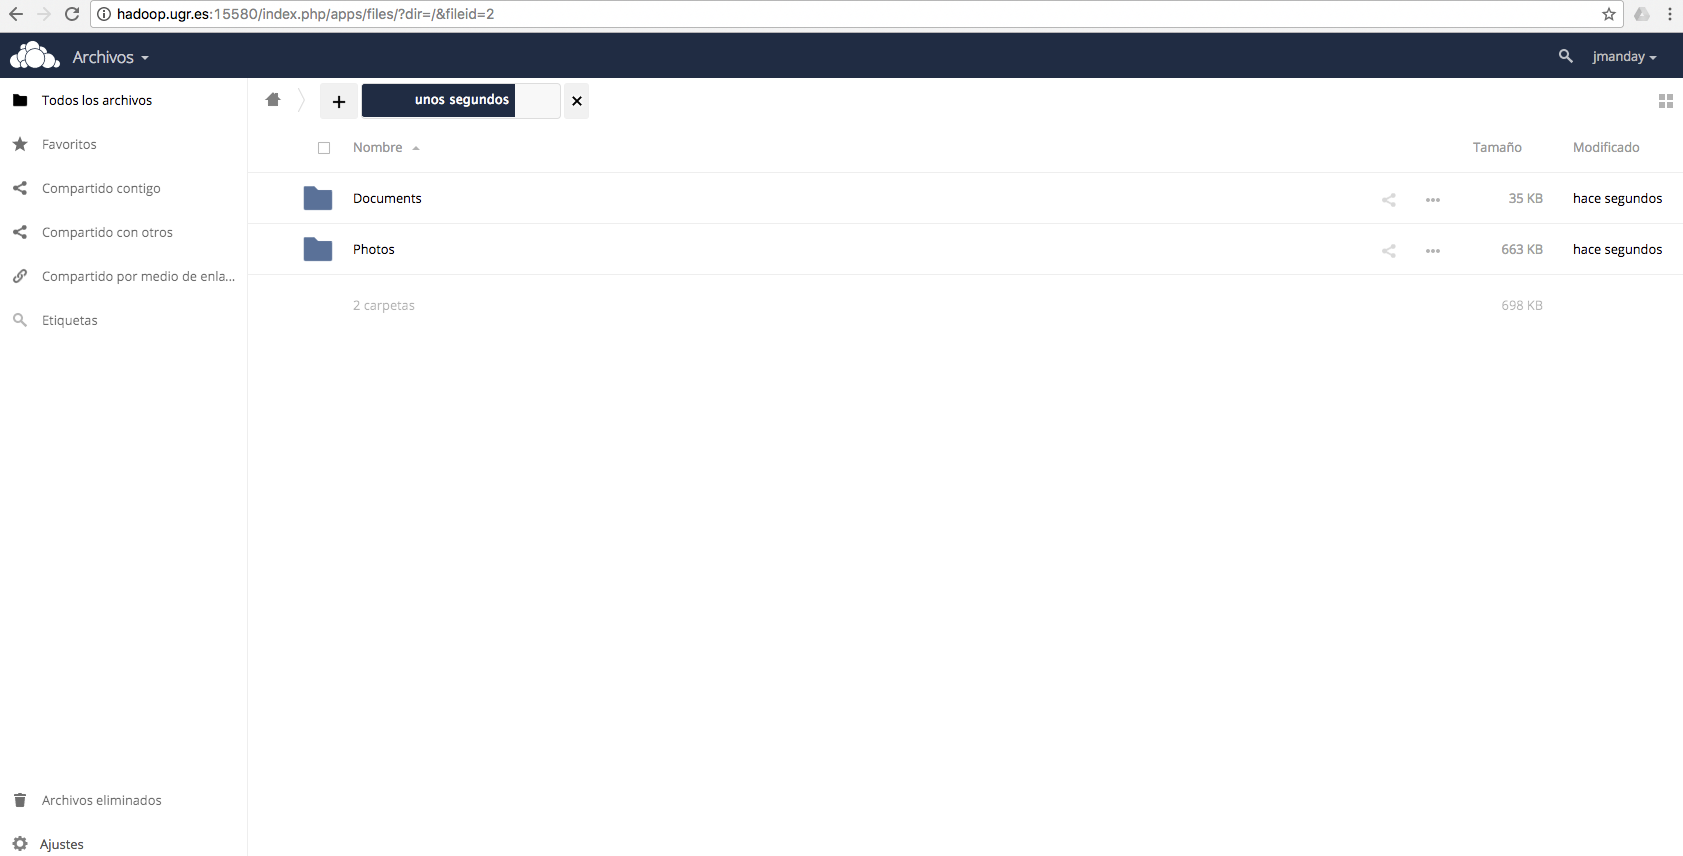
\includegraphics[width = 0.75\textwidth]{p2-img29}
 		\captionof{figure}{\label{fig:IPN}Probando ownCloud (II).} 
	\end{center} 
\end{figure}

  \begin{figure}[H]
	\begin{center}
 		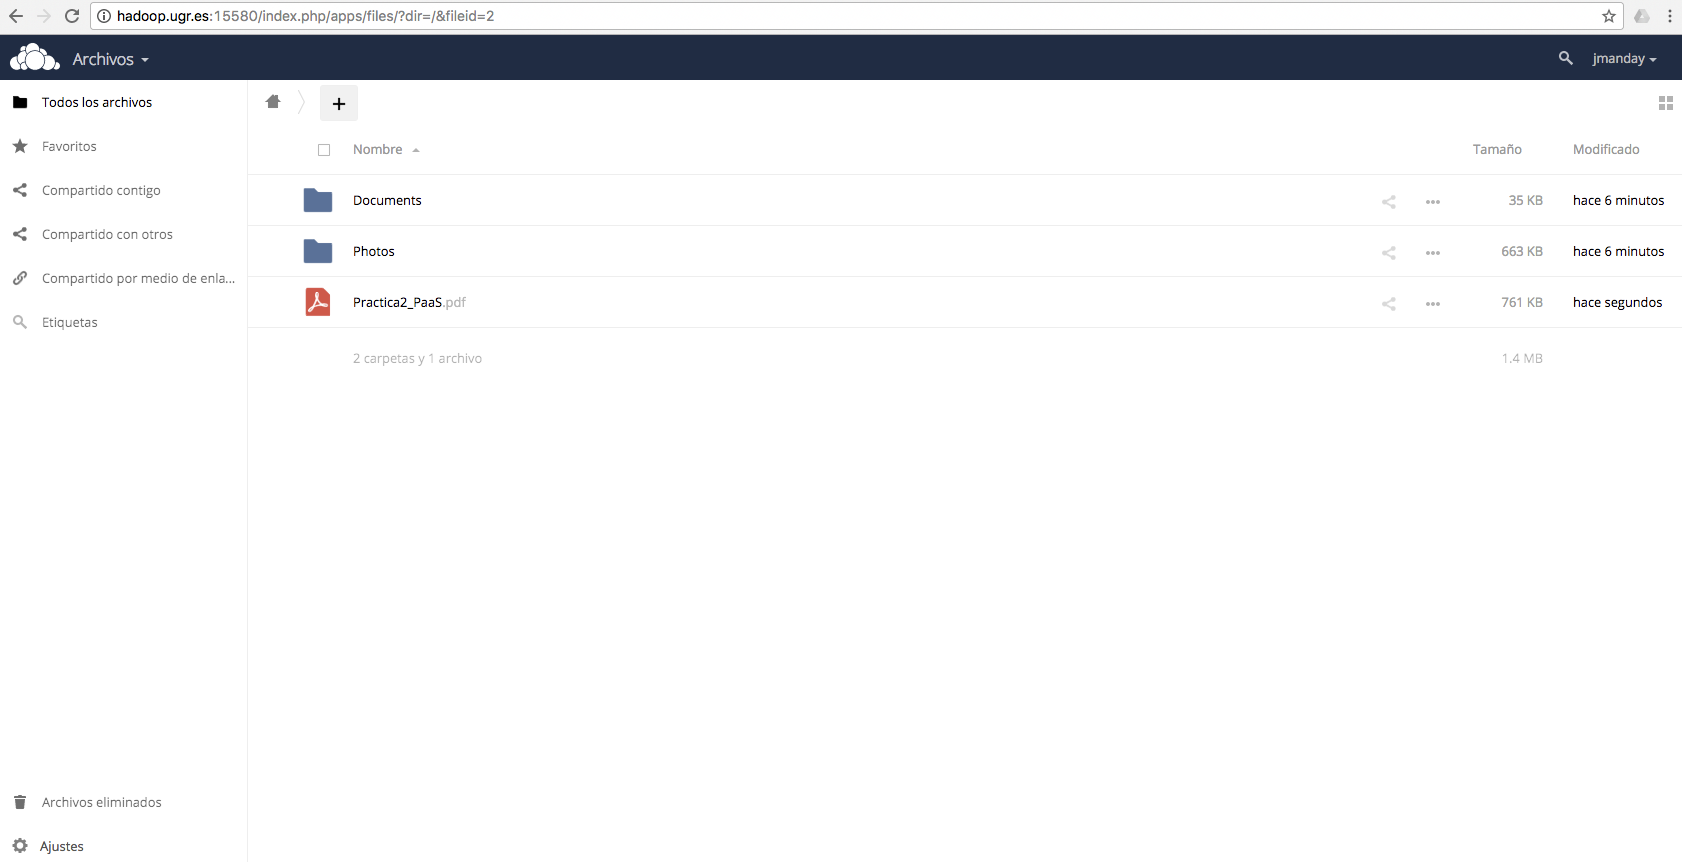
\includegraphics[width = 0.75\textwidth]{p2-img30}
 		\captionof{figure}{\label{fig:IPN}Probando ownCloud (III).} 
	\end{center} 
\end{figure}




\end{document}